\chapter{Abstract representation theory}
In this chapter, a ring will be a non necessarily commutative ring with unit.
\section{Semisimple rings}
\subsection{Definition and examples}
First we give some examples of noncommutative rings.
\begin{example}[\textbf{Examples of noncommutative rings}]
\mbox{}
\begin{itemize}
\item Let $R$ be a ring, then $\mathcal{M}_n(R)$ ($n\times n$ matrices with coefficients in $R$) is a noncommutative ring.
\item The \textbf{free $\bm{A}$-algebra} over a set $X$, where $A$ is a commutative ring, is the $A$-algebra $A\langle X\rangle$ of noncommutative polynomials with indeterminates in $X$. In other words, it's the algebra of the monoid $M_X$ whose elements are words on the elements of $X$ and whose multiplication is concatenation. This $M_X$ is called the \textbf{free monoid} on $X$.
\item Let $G$ be a group, the \textbf{group algebra} $R[G]$ of a group $G$ with coefficients in a (not necessarily commutative) ring $R$. As a $R$-module, this is the free $R$-module with basis $G$, that is, $R[G]=\bigoplus_{g\in G}Rg$. The multiplication is induced by that of $G$, i.e. given by:
\[\Big(\sum_{g\in G}\alpha_gg\Big)\Big(\sum_{g\in G}\beta_gg\Big)=\sum_{g\in G}\Big(\sum_{h_1h_2=g}\alpha_{h_1}\beta_{h_2}g\Big).\]
Note that this definition also makes sense if $G$ is a monoid.
\end{itemize}
\end{example}
Now we extend some notations in commutative rings that fits into the noncommutative case and will be used later.
\begin{definition}
Let $R$ be a ring. A \textbf{left (resp. right) $\bm{R}$-module} is a commutative group $M$
with a biadditive map $\rho:R\times M\to M$ such that:
\begin{itemize}
\item $\rho(1,x)=x$ for all $x\in M$.
\item $\rho(ab,x)=\rho(a,\rho(b,x))$ for all $a,b\in R$ and $x\in M$.
\end{itemize}
If we want to make it very clear that $M$ is a left (resp. right) $R$-module, we write $_{R}M$ (resp. $M_R$) instead of $M$. By convention, a $R$-module will be a left $R$-module unless otherwise specified.
\end{definition}
\begin{example}
The ring $R$ with left (resp. right) multiplication by itself is a left (resp. right) $R$-module, called the \textbf{left (resp. right) regular $\bm{R}$-module} and sometimes denoted by $R_R$ (resp. $_{R}R$).
\end{example}
\begin{definition}
Let $M$ be a $R$-module. A $R$-submodule (or submodule if $R$ is clear) of $M$ is a subgroup $N$ of $M$ such that $ax\in N$ for every $a\in R$ and $x\in N$.
\end{definition}
For example, a submodule of $_{R}R$ is just a left ideal of $R$.
\begin{definition}
If $M$ is a $R$-module and $N$ is a submodule of $M$, then the quotient group
$M/N$ has a structure of $R$-module. This is called a \textbf{quotient $\bm{R}$-module}.
\end{definition}
\begin{definition}
Let $M$ be a $R$-module and $(M_i)_{i\in I}$ be a family of submodules of $M$. We say that $M$ is the \textbf{sum} of the $M_i$ and write $M=\sum_{i\in I}M_i$ if, for every $x\in M$, there exist $x_i\in M$ such that $x=\sum_{i\in I}x_i$. We say that $M$ is the \textbf{direct sum} of the $M_i$ and write $M=\bigoplus_{i\in I}M_i$ if, for every $x\in M$, the $x_i$'s such that $x=\sum_{i\in I}x_i$ are uniquely determined.
\end{definition}
Let $M,N$ be two $R$-modules. Then we write $\Hom_R(M,N)$ for the abelian group of $R$-linear maps from $M$ to $N$. We also write $\End_R(M)$ for $\Hom_R(M,M)$; this is a ring, and its group of invertible elements will be denoted by $\Aut_R(M)$.
\begin{definition}
An \textbf{exact sequence} of $R$-modules is an exact sequence of abelian groups where all the abelian groups are $R$-modules and all the maps are $R$-linear.
\end{definition}
\begin{example}
\mbox{}
\begin{itemize}
\item $R^n$, seen as the set of $n\times1$ matrices with coefficients in $R$, is a left $\mathcal{M}_n(R)$-module with the operation given by matrix multiplication. If we see $R^n$ as the set of $1\times n$ matrices with coefficients in $R$, we similarly get a right $R$-module structure on it.
\item Let $A$ be a commutative ring. Then a $A[T]$-module is a $A$-module $M$ with a $A$-linear endomorphism. (It is the action of $T\in A[T]$ on $M$)
\item More generally, if $A$ is a commutative ring and $I$ is a set, then a $A[T_i,i\in I]$-module is a $A$-module $M$ with a family $(u_i)_{i\in I}$ of pairwise commuting $A$-linear endomorphisms. (The endomorphism $u_i$ is given by the action of $T_i$ on $M$.)
\item If $A$ is a commutative ring and $X$ is a set, then a $A\langle X\rangle$-module is a $A$-module $M$ with a family $(u_x)_{x\in X}$ of $A$-linear endomorphisms. (They are not required to commute with each other anymore.)
\item If $A$ is a commutative ring and $G$ is a group (or just a monoid), then a \textbf{$\bm{A[G]}$-module} is a $A$-module with a morphism of groups (or monoids) $G\to\Aut_A(M)$. This is also called a \textbf{$\bm{A}$-linear representation of the group (or monoid) $\bm{G}$} on the $A$-module $M$.
\end{itemize}
\end{example}
\subsection{Semisimple modules and rings}
\begin{example}
Let $k$ be a field and $M$ be a $k[T]$-module such that $\dim_k(M)<+\infty$. Then $M$ is a semisimple $k[T]$-module if and only if the endomorphism of $M$ given by the action of $T$ is diagonalizable over an algebraic closure of $k$.
\end{example}
\begin{remark}
A left ideal $I$ of $R$ is a simple $R$-module if and only if it is minimal
among nonzero left ideals of $R$. So if $R$ is a semisimple ring, it has minimal nonzero left ideals, moreover, $R$ is the direct sum of its minimal left ideals by Theorem~\ref{semisimple module iff}.
\end{remark}
To finish this subsection, we prove an intersting result about a left ideal of a semisimple ring.
\begin{proposition}\label{split left ideal principal}
Assume that $I$ is a left ideal of $R$, and that the short exact sequence 
\[\begin{tikzcd}
0\ar[r]&I\ar[r]&R\ar[r]&R/I\ar[r]&0
\end{tikzcd}\]
splits, that is, that there exists a left ideal $J$ of $R$ such that $R=I\oplus J$. Write $1=e_1+e_2$ with $e_1\in I$ and $e_2\in J$. Then 
\[e_1^2=e_1,\quad e_2^2=e_2,\quad e_1e_2=e_2e_1=0.\]
Also, $I=Re_1$ and $J=Re_2$.\par
If moreover $I$ and $J$ are ideals, then $IJ=0$, $e_1$ and $e_2$ are central in $R$, $I$ and $J$ and rings with respective units $e_1$ and $e_2$, and $R=I\times J$ as rings.\par
In particular, in a semisimple ring every left ideal is principal and generated by an idempotent.
\end{proposition}
\begin{proof}
We have 
\[e_1=e_1(e_1+e_2)=e_1^2+e_1e_2\]
and so $e_1-e_1^2=e_1e_2\in I\cap J$. Then this implies $e_1^2=e_1$ and $e_1e_2=0$. Similarly, $e_2^2=e_2$ and $e_2e_1=0$.\par 
Obviously, $Re\sub I$; conversely, if $x\in I$, then $x=x(e_1+e_2)=xe_1+xe_2$, so $x=xe_1\in Re_1$ and $xe_2=0$. This shows that $I=Re$. The proof that $J=Re_2$ is similar.\par
Assume that $I$ and $J$ are ideals. The $IJ\sub I\cap J=0$. Let $a\in R$, then
\[a=a(e_1+e_2)=ae_1+ae_2=(e_1+e_2)a=e_1a+e_2a\]
As $R=I\oplus J$, we have $ae_1=e_1a$ and $ae_2=e_2a$. If moreover $a\in I$ (resp. $a\in J$), then $ae_1=e_1a=a$ and $ae_2=e_2a=0$ (resp. $ae_1=e_1a=0$ and $ae_2=e_2a=1$).\par
To finish the proof, let's show that the map 
\[\varphi:I\times J\to R,\quad (a,b)\mapsto a+b\]
is an isomorphism of rings. We already know that it is an isomorphism of abelian groups by hypothesis. Let $a,a'\in I$ and $b,b'\in J$. Then
\[\varphi(a,b)\varphi(a',b')=(a+b)(a'+b')=aa'+bb'=\varphi((a,b)(a',b')).\]
Thus the cliam follows.
\end{proof}
\subsection{Schur's lemma}
The following result is the most important property for simple modules, so we rule out it.
\begin{theorem}[\textbf{Schur's lemma}]
Let $R$ be a ring, $M$ and $N$ be $R$-modules, and $\varphi:M\to N$ be a $R$-linear map.
\begin{itemize}
\item If $M$ is simple, then $\varphi=0$ or $\varphi$ is injective.
\item If $N$ is simple, then $\varphi=0$ or $\varphi$ is surjective.
\item If $M$ and $N$ are simple, then $\varphi=0$ or $\varphi$ is an isomorphism.
\end{itemize}
In particular, if $M$ is a simple $R$-module, then $\End_R(M)$ is a division ring.
\end{theorem}
\begin{proof}
This follows from the fact that $\ker\varphi$ is a submodule of $M$ and $\im\varphi$ is a submodule of $N$.
\end{proof}
\begin{corollary}
Let $\varphi:M\to N$ be a homomorphism of $A$-modules. If $M$ is semisimple, then $\im\varphi$ is also semisimple.
\end{corollary}
\begin{proof}
Let $M=\sum_{i\in I}S_i$ with $S_i$ simple. By Schur's lemma, $\varphi|_{S_i}:S_i\to N$ is either $0$ or injective. Hence $\varphi(S_i)$ is either $0$ or is isomorphic to $S_i$ and therefore simple. Since $\im\varphi=\sum_{i\in I}\varphi(S_i)$, it follows that $\im\varphi$ is semisimple.
\end{proof}
\subsection{Jordan-H\"older theorem}
\begin{definition}
Let $R$ be a ring and $M$ be a $R$-module.
\begin{itemize}
\item A \textbf{Jordan-H\"older series} (or \textbf{composition series}) for $M$ is a sequence of submodules
\[M=M_0\supset M_1\supset\cdots\supset M_n=0\]
of $M$ such that $M_i/M_{i+1}$ is a simple $R$-module for every $i$. We say that the integer $n$ is the \textbf{length} of the series.
\item If a composition series for $M$ exists, we say that $M$ is has finite length. Then the length $\ell(M)$ of $M$ is the minimum of the lengths of all its Jordan-H\"older series. If $M$ is not of finite length, we set $\ell(M)=+\infty$.
\item Two Jordan-H\"older series $(M_i)_{0\leq i\leq n}$ and $(M'_i)_{0\leq i\leq m}$ are called \textbf{equivalent} if $n=m$ and there exists a permutation $\sigma\in\mathfrak{S}_n$ such that $M_i/M_{i+1}\cong M'_{\sigma(i)}/M'_{\sigma(i+1)}$ for every $i$.
\end{itemize}
\end{definition}
\begin{lemma}
Suppose as above that $M$ has finite length, and let $N$ be a submodule of $M$. Then $N$ and $M/N$ have finite length, and in fact $\ell(N)\leq\ell(M)$ and $\ell(M/N)\leq\ell(M)$.
\end{lemma}
\begin{theorem}[\textbf{Jordan-H\"older}]
If $M$ has finite length, then all its Jordan-H\"older series are equivalent. In particular, all the Jordan-H\"older series of $M$ have the same length, and the length of $M$ is the length of any of its Jordan-H\"older series.
\end{theorem}
This theorem justifies the following definition:
\begin{definition}\label{module length quotient}
If M has finite length qnd $(M_i)$ is a Jordan-H\"older series for $M$, then the simple $R$-modules $M_i/M_{i+1}$, counted with multiplicities, are called the \textbf{Jordan-H\"older constituents} of $M$.
\end{definition}
\begin{corollary}
If $M$ has finite length and $N$ is a submodule of $M$, then the Jordan-H\"older factor of $M$ are exactly those of $N$ and $M/N$, and we have $\ell(M)=\ell(N)+\ell(M/N)$.
\end{corollary}
\subsection{Artinian and Noetherian modules}
\begin{definition}
Let $R$ be a ring.
\begin{itemize}
\item We say that a $R$-module $M$ is \textbf{Artinian} (resp. \textbf{Noetherian}) if every strictly decreasing (resp. strictly increasing) sequence of submodules of $M$ is finite.
\item We say that $R$ is \textbf{left Artinian} (resp. \textbf{left Noetherian}) if the left $R$-module $_{R}R$ is Artinian (resp. Noetherian).
\end{itemize}
\end{definition}
Now we prove that a module has finite length if and only if it is both Artinian and Noetherian. First we need a lemma.
\begin{lemma}
Let $M$ be a $R$-module.
\begin{itemize}
\item If $M\neq 0$ and $M$ is Artinian (resp. Noetherian), then it admits minimal (resp. maximal) nonzero submodules.
\item If $M$ is Artinian (resp. Noetherian), so is any submodule and any quotient of $M$ is Noetherian.
\end{itemize}
\end{lemma}
\begin{proposition}\label{module finite length iff}
Let $M$ be a $R$-module. Then $M$ has finite length if and only if it is both
Artinian and Noetherian.
\end{proposition}
\begin{proof}
Suppose that $M$ is Artinian and Noetherian. Let's prove that $M$ has finite length. We construct by induction on $i$ a sequence $(M_i)_{i\in\N}$ of submodules of $M$ such that, for every $i\in\N$, $M_i\sub M_{i+1}$ and $M_{i+1}/M_i$ is zero or simple.\par
Take $M_0=0$. Now suppose that $i\geq0$ and that $M_0,\dots,M_{i+1}$ are constructed. If $M_i=M$, take $M_{i+1}=M_i$. Otherwise, then by the fact that $M$ is Artinian and by the lemma, $M/M_i$ has a minimal nonzero submodule, and we take for $M_{i+1}$ its inverse image in $M$. By minimality of $M_{i+1}/M_i$, this $R$-module is simple.\par
We also know that $M$ is Noetherian, so the sequence $(M_i)$ must stabilize toM after a finite number of steps. As all the quotients $M_{i+1}/M_i$ are wero or simple, we can extract from $(M_i)$ a Jordan-H\"older sequence for $M$, and so $M$ has finite length.\par
Now suppose that $M$ has finite length, and let's prove that $M$ is Artinian and Noetherian. If $M$ is not Noetherian, then it has an infinite sequence of submodules $M_0\sub M_1\sub\cdots$. But then $\ell(M_{i+1})\leq\ell(M_i)+1$ for every $i\in\N$, so $\ell(M_i)\geq i$, so $\ell(M)$ cannot be finite. Similarly, we see that if $M$ is not Artinian, then it cannot have finite length.
\end{proof}
\begin{example}
If $k$ is a field and $R$ is a $k$-algebra that is finite-dimensional as a $k$-vector space, then $R$ is left Artinian and left Noetherian. (Because every left ideal of $R$ is a $k$-vector subspace.)
\end{example}
Now we connect semisimple rings with the properties.
\begin{proposition}\label{semisimple ring Art Noe}
If $R$ is a semisimple ring, then $R$ is left Artinian and left Noetherian.
\end{proposition}
\begin{proof}
By Theorem~\ref{semisimple module iff}, $R=\bigoplus_{i\in I}I_i$, where the $I_i$ are left ideals of $R$ that are simple as $R$-modules. If we show that $I$ is finite, then $_{R}R$ will have finite length, hence be an Artinian and Noetherian $R$-module, and we will be done. To show
that $I$ is finite, write $1=\sum_{i\in I}x_i$, with $x_i\in I_i$ for every $i\in I$ and $x_i=0$ for all but a finite number of $i$'s. Then it can be seen that $R$ is generated by these $x_i$'s, so $I$ is finite.
\end{proof}
\subsection{Isotypic decomposition}
Let $R$ be a ring. We write $S(R)$ for the set of isomorphism classes of simple $R$-modules. In this subsection we want to decompose $R$ as a direct sum of simple modules, as stated in Theorem~\ref{semisimple module iff}.\par
The following lemma will be used repeatedly in the proof of the next theorem.
\begin{lemma}\label{module sum of simple}
Let $M$ be a $R$-module, and suppose that there exists a simple $R$-module $S$ and a set $I$ and an isomorphism $\varphi:M\stackrel{\sim}{\to}\bigoplus_{i\in I}S$. Then every simple $R$-submodule of $M$ is isomorphic to $S$.
\end{lemma}
\begin{proof}
Let $N$ be a simple $R$-submodule of $M$, and suppose that $N$ is not isomorphic to $S$. Then for every $i\in I$, the composition of the projection on the $i$-th summand $\bigoplus_{i\in I}S\to S$ and of $\varphi$ is a $R$-linear map $N\to S$, which has to be zero by Schur's lemma. But then $\varphi$ is zero on $N$, which implies that $N=0$, contradicting the fact that $N$ is simple.
\end{proof}
Now we present our main thoerem.
\begin{theorem}\label{isotypic decomp}
Let $R$ be a ring and $M$ be a semisimple $R$-module. For every $S\in S(R)$, let $M_S$ be the sum of all the submodules of $M$ that are isomorphic to $S$. Then:
\begin{itemize}
\item[$(1)$] We have $M=\bigoplus_{S\in S(R)}M_S$.
\item[$(2)$] There exist a set $I_S$ such that $M_S\cong\bigoplus_{i\in I_S}S$ for every $S\in S(R)$. Therefore the decomposition of $M$ can be written into
\[M=\bigoplus_{S\in S(R)}S^{I_S}.\]
\item[$(3)$] Let $N$ be a submodule of $M$. If we write $N\cong\bigoplus_{S\in S(R)}N_S$ and $N_S\cong\bigoplus_{i\in J_S}S$, then, for every $S\in S(R)$, $N_S=M_S\cap N$ for every $S\in S(R)$ and we can find an injection $J_S\hookrightarrow I_S$.
\end{itemize}
\end{theorem}
The nonzero $M_S$ are called the \textbf{isotypic components} of $M$, and $M=\bigoplus_{S\in S(R)}M_S$ is called the \textbf{isotypic decomposition} of $M$. If $I_S$ is a finite set for some $S\in S(R)$, we call $|I_S|$ the \textbf{multiplicity} of $S$ in $M$.
\begin{proof}
First, note that $\bigoplus_{S\in S(R)}M_S$ is the sum of all the simple submodules of $M$. As $M$ is semisimple, $\bigoplus_{S\in S(R)}M_S$. Now we want to show that the sum is direct. Let $S\in S(R)$, let $\mathcal{X}=S(R)-\{S\}$. We must show that $N:=M_S\cap(\sum_{S'\in\mathcal{X}}M_{S'})=0$. As $N$ is submodule of $M$, it is semisimple, so, if it's nonzero, then it has a simple submodule $N'$. But then $N'$ is a simple submodule of both $N$ and $\sum_{S'\in\mathcal{X}}M_{S'}$, hence is isomorphic to $S$ and to an element of $\mathcal{X}$. This is not possible. So $N=0$.\par
As $M_S$ is a submodule of the semisimple $R$-module $M$, it is semisimple. By Theorem~\ref{semisimple module iff}, $M_S$ is the direct sum of a family of simple submodules. But every simple submodules of $M_S$ is isomorphic to $S$.\par
Let $S\in S(R)$. Then $N_S$ is a sum of simple $R$-modules isomorphic to $S$, so $N_S\sub M_S$. On the other hand, $N\cap M_S$ is a direct sum of simple submodules of $N$, and all these simple modules have to be isomorphic to $S$, so $N_S=N\cap M_S$.\par
So we may assume that $M=M_S$ and $N=N_S$ for some $S\in S(R)$, and we are reduced to the following statement.
\end{proof}
\begin{proposition}
If $S$ is a simple $R$-module and $I,J$ are two sets such that we have an injective $R$-linear map 
\[\varphi:N:=\bigoplus_{j\in J}S\to\bigoplus_{i\in I}S=:M,\]
then there exists an injection $J\hookrightarrow I$. 
\end{proposition}
We will only use this statement when $I$ and $J$ are finite, and in that case it follows from the Jordan-H\"older theorem, but let's see how to prove it general.
\begin{proof}
For any $R$-modules $M_1,M_2$, let $\Hom_{fl}(M_1,M_2)\sub\Hom_R(M_1,M_2)$ be the subgroup of $R$-linear maps that are $0$ outside a finite length submodule of $M_1$. Then we have
\[\Hom_{fl}(N,S)=\bigoplus_{j\in J}\End_R(S)\sub\Hom_R(N,S)=\prod_{j\in J}\End_R(S).\]
\[\Hom_{fl}(M,S)=\bigoplus_{i\in I}\End_R(S)\sub\Hom_R(M,S)=\prod_{i\in I}\End_R(S).\]
Note that $D:=\End_R(S)$ is a division ring by Schur's lemma, that $\Hom_R(M,S)$ and $\Hom_R(N,S)$ are naturally $D$-modules and that $\Hom_{fl}(M,S)$ and $\Hom_{fl}(N,S)$ are $D$-submodules. Moreover, we have a map
\[\varPhi:\Hom_{fl}(M,S)\to\Hom_{fl}(N,S)\quad f\mapsto f\circ\varphi\]
and it is clearly $D$-linear. If we can show that $\varPhi$ is surjective, we will done by linear algebra. So let $g\in\Hom_{fl}(N,S)$. As $M$ is a semisimple $R$-module, there exists a $R$-submodule $N'$ of $M$ such that $M=\varphi(N)\oplus N'$. Define $f:M\to S$ by 
\[f(\varphi(x)+y)=g(x)\for x\in N,y\in N'.\]
This makes sense because $\varphi$ is injective, is clearly $R$-linear, and we have $\varPhi(f)=g$.
\end{proof}
\subsection{Simple rings}
Before we proceed to the formulation of the Wedderburn-Artin Theorem, it will be useful to first construct some examples of left semisimple rings.
The only obvious example so far is that of a division ring. If $D$ is a division ring, then its left modules are the left vector spaces over $D$. It is well-known that any short exact sequence of vector spaces splits, so $D$ is semisimple. To produce more examples, we shall use the construction of finite matrix rings. First let us prove the following elementary result on
the classification of ideals in a matrix ring.
\begin{definition}
A ring $R$ is called \textbf{simple} if $R\neq0$ and if the only ideals of $R$ are $0$ and $R$.
\end{definition}
\begin{remark}
Note that the definition of a simple ring involves ideals, and that of a semisimple ring involves left ideals. In particular, a simple ring has no a priori reason to be semisimple, and indeed there exist simple rings that are not semisimple. So the terminology is a bit unfortunate.
\end{remark}
\begin{proposition}
If $R$ is a ring and $n\geq1$ is an integer, then any ideal $I$ of $\mathcal{M}_n(R)$ if of the form $I=\mathcal{M}_n(J)$, where $J$ is a uniquely determined ideal of $R$. In particular, if $R$ is a simple ring, so is $\mathcal{M}_n(R)$.
\end{proposition}
\begin{proof}
If $J$ is an ideal of $R$, then $\mathcal{M}_n(J)$ is clearly an ideal of $\mathcal{M}_n(R)$. Also, if $J,J'$ are two ideals of $R$ such that $\mathcal{M}_n(J)=\mathcal{M}_n(J')$, then it is obvious that $J=J'$. So we just need to prove that any ideal of $\mathcal{M}_n(R)$ is of the form $\mathcal{M}_n(J)$.\par
Let $I$ be an ideal of $\mathcal{M}_n(R)$, and let $J$ be the set of $(1,1)$-entries of elements of $I$. We'll show that $J$ is an ideal and that $I=\mathcal{M}_n(J)$.\par
First, let $x,y\in J$ and let $a\in R$. Choose matrices $X,Y\in I$ such that the $(1,1)$-entries of $X$ and $Y$ are $x$ and $y$ respectively. Then $aX$, $Xa$ and $X+Y$ are in $I$, and their respective $(1,1)$-entries are $ax,xa$ and $x+y$. So $J$ is an ideal of $R$.\par
Now let's denote by $E_{ij}$, for $1\leq i,j\leq n$, the elementary matrices in $\mathcal{M}_n(R)$. If $X=(x_{ij})\in\mathcal{M}_n(R)$, then we have the identity
\[E_{ij}XE_{kl}=x_{jk}E_{jk}\]
If $X\in I$, then for all $j,k$ we have $E_{1j}XE_{k1}=x_{jk}E_{11}\in I$, so $x_{jk}\in J$, and so $X\in\mathcal{M}_n(J)$. Conversely, take any $X=\sum_{ij}x_{ij}E_{ij}\in\mathcal{M}_n(J)$, to show that $X\in I$, it suffices to show all the $x_{ij}E_{ij}$ are in $I$. Fix $i$ and $j$ and choose $Y\in I$ such that the $(1,1)$-entry of $Y$ is $x_{ij}$, then $E_{i1}YE_{1j}=x_{ij}E_{ij}\in I$.
\end{proof}
In the next theorem, we study in detail the properties of a matrix ring
over a division ring.
\begin{theorem}\label{division matrix ring}
Let $D$ be a division ring, and let $R=\mathcal{M}_n(D)$, $V=D^n$. Then
\begin{itemize}
\item[$(1)$] $R$ is simple, semisimple, left artinian and left noetherian.
\item[$(2)$] $V$ is the unique left simple module of $R$ (up to isomorphism). $R$ acts faithfully on $V$, and we have $_{R}R\cong V^n$ as $R$-modules.
\item[$(3)$] $\End_D(V_D)=R$ and $\End_R(_{R}V)=D$.
\end{itemize}
\end{theorem}
\begin{proof}
Let's prove $(1)$. First, by the proposition, $R$ is simple because $D$ is. As a left $D$-vector space, $R$ is finite-dimensional. Since left ideals of $R$ are $D$-vector subspaces of $R$, $R$ is left Artinian and left Noetherian.\par
Let’s prove that $_{R}V$ is a simple $R$-module. Take a nonzero $R$-submodule $W$ of $_{R}V$. We use the same notation $E_{ij}$ as in the proof of the proposition. Let $w\in W-\{0\}$ and write $w=(w_1,\dots,w_n)^T$. Choose $i_0$ such that $w_{i_0}\neq 0$, then
\[\begin{pmatrix}
1\\
0\\
\vdots\\
0
\end{pmatrix}=(w_{i_0}^{-1}E_{1i_0})w\in W.\]
Now if $v=(v_1,\dots,v_n)^T$ is any element of $_{R}V$, then
\[\begin{pmatrix}
v_1&0&\cdots&0\\
\vdots&\vdots&&\vdots\\
v_n&0&\cdots&0
\end{pmatrix}\begin{pmatrix}
1\\
0\\
\vdots\\
0
\end{pmatrix}\in W\]
and so $V=W$. As the left $R$-module $_{R}R$ is clearly isomorphic to $_{R}V^n$, the ring $R$ is semisimple.\par
Let's prove $(2)$. It only remains to show that any simple $R$-module is isomorphic to $_{R}V$. But since $_{R}R\cong V^n$, this comes from Lemma~\ref{module sum of simple}.\par
Let's prove $(3)$. Consider the map 
\[\Delta:R\to\End_D(V_D),\quad A\mapsto(x\mapsto Ax).\]
This map is well-defined, because for every $A\in R,x\in V$ and $\lambda\in D$,
\[\Delta(A)(x\lambda)=A(x\lambda)=(Ax)\lambda=\Delta(A)(x)\lambda.\]
so $\Delta(A)$ is $D$-linear. The map $\Delta$ is easily seen to be an isomorphism of rings.\par
Now consider $E:=\End_R(_{R}V)$. We write the action of the ring $E$ on $V$ on the right: $v\cdot\varphi=\varphi(v)$ for $v\in V$ and $x\in E$. Let 
\[\Psi:D\to E,\quad \lambda\mapsto(x\mapsto x\lambda).\]
This map is well-defined, i.e. $\Psi(\lambda)$ is $R$-linear for every $\lambda\in D$, and it is a morphism of rings. We want to show that it is an isomorphism of rings. First, $\Psi$ is injective because $n\geq1$ and $D$ is a division algebra. Now let $\varphi\in E$. Define $\lambda\in D$ by
\[e_1\cdot\varphi=\lambda e_1+\sum_{j=2}^{n}\mu_je_j,\quad \mu_j\in D\]
where $e_1,\dots,e_n$ are standard basis of $V$. Let $v=(v_1,\dots,v_n)^T\in V$ and
\[A=\begin{pmatrix}
v_1&0&\cdots&0\\
\vdots&\vdots&&\vdots\\
v_n&0&\cdots&0
\end{pmatrix}\in R.\]
Then $Ae_1=v$ and
\[v\cdot\varphi=(Ae_1)\cdot\varphi=A(e_1\cdot\varphi)=A\begin{pmatrix}
\lambda\\
\mu_2\\
\vdots\\
\mu_n
\end{pmatrix}=\begin{pmatrix}
v_1\lambda\\
\vdots\\
v_n\lambda
\end{pmatrix}=v\lambda,\]
where we use $\varphi$ is $R$-linear. So $\varphi=\Psi(\lambda)$ and $\Psi$ is surjective.
\end{proof}
\begin{corollary}\label{division matrix ring unique}
If $D,D'$ are two division rings and $n,n'\geq1$ are two integers such that
$\mathcal{M}_n(D)\cong\mathcal{M}_{n'}(D')$ as rings, then $D\cong D'$ and $n=n'$.
\end{corollary}
\begin{proof}
Let $R=\mathcal{M}_n(D)\cong\mathcal{M}_{n'}(D')$, and let $V$ be the unique simple $R$-module. By $(3)$ of the theorem, $D'\cong\End_R(_{R}V)\cong D$. Hence
\[n=\dim_D(V)=\dim_{D'}(V)=n',\]
and we are done.
\end{proof}
\subsection{Artin-Wedderburn theorem}
In order to produce more examples of semisimple rings, we make the following observation on finite direct products of rings.
\begin{proposition}\label{submodule product ring}
Let $R_1,\dots,R_n$ be rings, and let $R=R_1\times\cdots\times R_n$. Then every $R$-module is of the form $M=M_1\times\cdots\times M_n$, with $M_i$ a $R_i$-module for $1\leq i\leq n$.
\end{proposition}
\begin{proof}
In $R$, write $1=e_1+\cdots+e_n$, with $e_i\in R_i$. Of course, as an element of $R_1\times\cdots\times R_n$, $e_i$ is the $n$-uple with $i$-th entry equal to $1\in R_i$ and all the other entries equal to $0$. Note that all the $e_i$ are central in $R$, that $e^2_i=e_i$ for every $i$ and that $e_ie_j=e_je_i=0$ for $i\neq j$.\par
Let $M$ be a $R$-module, set $M_i=e_iM$. Then $R$ acts on $M_i$ through the obvious projection $R\to R_i$, so we just need to show that $M\cong M_1\times\cdots\times M_n$. Consider the map
\[\varPhi:M_1\times\cdots\times M_n\to M,\quad (x_1,\dots,x_n)\mapsto x_1+\cdots+x_n.\]
This is a $R$-linear map by the previous remark about the action of $R$ on the $M_i$. If $x\in M$, then $x=e_1x+\cdots+e_nx$ with $e_ix\in M_i$ for every $i$, so $\varPhi$ is surjective. Moreover, if $x_1+\cdots+x_n=0$ with $x_i\in M_i$ for every $i$, then for every $j\in\{1,\dots,n\}$ we have 
\[0=e_j(x_1+\cdots+x_n)=e_jx_j=x_j.\] 
Hence $\varPhi$ is injective.
\end{proof}
\begin{corollary}\label{simple module product ring}
Suppose that $R=R_1\times\cdots\times R_n$.
\begin{itemize}
\item $R$ is semisimple if and only if all the $R_i$ are semisimple.
\item Every simple $R$-module is of the form $0\times\cdots\times0\times M_i\times0\times\cdots\times 0$, with $i\in\{1,\dots,n\}$ and $M_i$ a simple $R_i$-module.
\end{itemize}
\end{corollary}
\begin{proof}
Let $M$ be a $R$-module, then $M=M_1\times\cdots\times M_n$ with $M_i$ a $R_i$-module. Since $R_i$ are semisimple, each $M_i$ is semisimple and hence is a direct sum of simple $R_i$-modules:
\[M_i=\bigoplus_{j=1}^{n_i}M_{ij}\for i\in\{1,\dots,n\}.\]
Then we see that
\[M=\bigoplus_{i=1}^{n}M_i=\bigoplus_{ij}M_{ij}\]
is also semisimple.
\end{proof}
\begin{corollary}
Let $D_1,\dots,D_r$ be division rings, and $n_1,\dots,n_r\geq1$ be integers. Then $R:=\mathcal{M}_{n_1}(D_1)\times\cdots\times\mathcal{M}_{n_r}(D_r)$ is a semisimple ring, and its simple modules (up to isomorphism) are $D_1^{n_r},\dots,D_r^{n_r}$.
\end{corollary}
This gives a good stock of examples of semisimple rings. Remarkably, it turns out that these are all the examples! This is the content of the following celebrated result.
\begin{theorem}[\textbf{Wedderburn-Artin Theorem}]\label{Wedderburn-Artin}
Let $R$ be any semisimple ring. Then for suitable division rings $D_1,\dots,D_r$ and positive integers $n_1,\dots,n_r$ we have \[R\cong\mathcal{M}_{n_1}(D_1)\times\cdots\times\mathcal{M}_{n_r}(D_r)\]
The pairs $(n_1,D_1),\dots,(n_r,D_r)$ are uniquely determined up to a permutation. There are exactly $r$ mutually nonisom orphic left simple modules over $R$.
\end{theorem}
\begin{proof}
Let $R$ be a semisimple ring. Decompose $_{R}R$ into a finite direct sum of minimal left ideals. Grouping these according to their isomorphism types as left $R$-modules, we can write
\[_{R}R=n_1V_1\oplus\cdots\oplus n_rV_r.\]
where $V_1,\dots,V_r$ are mutually nonisomorphic simple left $R$-modules. If $V$ is any simple left $R$-module, $V$ is isomorphic to a quotient of $_{R}R$ and hence by the Jordan-H\"older Theorem isomorphic $V_i$. Therefore $\{V_1,\dots,V_r\}$ is a full set of mutually nonisomorphic left simple $R$-modules.\par
Now we have
\[_{R}R\cong\End_R(_{R}R)\cong\bigoplus_{i=1}^{r}\End_R(V_i^{n_i})=\bigoplus_{i=1}^{r}\mathcal{M}_{n_i}(\End_R(V_i))\]
Since the $\End_R(V_i)$ are division rings by Schur's lemma, existence is proved.\par
To prove the uniqueness of this decomposition, suppose we have another
isomorphism
\[R\cong\mathcal{M}_{n'_1}(D'_1)\times\cdots\times\mathcal{M}_{n'_r}(D'_r)\]
where $D'_1,\dots,D'_r$ are division rings. Let $V'_i$ be the unique simple left module over $\mathcal{M}_{n'_i}(D'_i)$. We can also view $V'_i$ as a simple left module over $R$; clearly $V'_i\ncong V'_j$ as $R$-modules if $i\neq j$. By Theorem~\ref{isotypic decomp} and Corollary~\ref{simple module product ring} we have
\[_{R}R\cong n'_1V'_1\oplus\cdots\oplus n'_rV'_r.\]
By the Jordan-Holder Theorem, we see that $r=s$ and that (upon reindexing) $n'_i=n_i$ and $V_i=V'_i$ for all $i$. Writing $R_i=\mathcal{M}_{n_i}(D_i)$, we have
\[D'_i\cong\End_{R_i}(V'_i)\cong\End_{R}(V'_i)\cong\End_{R}(V_i)=D_i\]
for all $i$.
\end{proof}
Note that the existence of an isomorphism
\[R\cong\mathcal{M}_{n_1}(D_1)\times\cdots\times\mathcal{M}_{n_r}(D_r)\]
amounts to the fact that there are ideals $R_1,\dots,R_r$ in $R$ such that $R=R_1\oplus\cdots\oplus R_r$ and that, as a ring, each $R_i$ is isomorphic to the simple ring $\mathcal{M}_{n_i}(D_i)$, The following general lemma on direct decompositions of a ring implies that the $R_i$'s are not only determined up to isomorphism as rings, but they are, in fact, uniquely determined as ideals in $R$. In the sequel, we shall call them the \textbf{simple components} of the (semisimple) ring $R$.
\begin{lemma}
Let $R$ be a ring with nonzero ideals $R_1,\dots,R_r$ and $R'_1,\dots,R'_s$ such that
\[R=R_1\oplus\cdots\oplus R_r=R'_1\oplus\cdots\oplus R'_s\]
and such that each $R_i$ as well as each $R'_j$ is indecomposable as an ideal (i.e., not a direct sum of two nonzero subideals). Then $r=s$, and after a permutation of indices we have $R_i=R'_j$.
\end{lemma}
\begin{proof}
Viewing the$R_i$'s as rings, $R\cong R_1\times\cdots\times R_r$. Under this isomorphism, the ideal $R'_1$ in $R$ corresponds to an ideal $I_1\times\cdots\times I_r$ where each $I_i$ is an ideal in $R_i$ (see Proposition~\ref{submodule product ring}). Since $R'_1$ is indecomposable as an ideal, all but one $I_i$ must be zero. After a permutation of indices, we may assume $I_2=\cdots=I_r=0$ and so $R'_1\sub R_1$. Similarly, we have $R_1\sub R'_i$ for some $i$. But then $R'_1\sub R'_i$ implies that $i=1$; hence $R'_1=R_1$. Repeating the same argument for the other $R_i$'s, we obtain the desired conclusion.
\end{proof}
Let $R$ be a semisimple ring. We know that $R$ has a finite number of uniquely determined simple components: they are minimal (two-sided) ideals in $R$, and $R$ is their direct sum. One may ask the following natural question: Is it possible to give a more \textbf{intrinsic construction} of these simple components? We shall show that this is indeed possible, even independently of the proof we have given for Theorem~\ref{Wedderburn-Artin}. In particular, the construction below provides a second route to the existence of the simple decomposition of $R$.\par
For any minimal left ideal $I$ in a ring $R$, let $\mathscr{I}_I$ be the sum of all the minimal left ideals of $R$ which are isomorphic to $I$ as left R-modules. The following general properties of $\mathscr{I}_I$ are valid without any assumptions on the ring $R$.
\begin{lemma}
Let $R$ be a ring and $I$ be a minimal nonzero left ideal of $R$. Then $\mathscr{I}_I$ is an ideal of $R$. Moreover, if $I$ and $J$ are two nonisomorphic minimal nonzero left ideals of $R$, then $\mathscr{I}_I\cdot\mathscr{I}_J=0$.
\end{lemma}
\begin{proof}
The main point is that minimal nonzero left ideals of $R$ are simple $R$-modules.\par
Let's prove that $\mathscr{I}_I$ is a right ideal. Let $I'$ be a left ideal of $R$ such that $I'\cong I$ as $R$-modules, and let $a\in R$. We want to show that $I'a\sub\mathscr{I}_I$. But $I'a$ is a homomorphic image of $I'$, and so we can only have $I'r=0$ or $I'r\cong I'\cong I$. In either case, $I'r\sub\mathscr{I}_I$.\par
Now let $J$ be another minimal nonzero left ideal of $R$, it is enough to show that $IJ=0$. Assume, on the contrary, that $Ia\neq0$ for some $a\in J$. Since $J$ is a minimal left ideal, we must have $Ia=J$. But then $I\cong Ia=J$ (as left $R$-modules), a contradiction.
\end{proof}
\begin{proposition}\label{semisimple finite dim ring}
Let $k$ be a field, and suppose that $R$ is a semisimple $k$-algebra that is finite-dimensional as a $k$-vector space. Then its simple factors $R_i$ are also $k$-algebras, and so are the division rings $D_i$. Moreover, each $D_i$ is finite dimensional over $k$.\par
In particular, if $k$ is algebraically closed, then all the $D_i$ are equal to $k$, so $R\cong\mathcal{M}_{n_1}(k)\times\cdots\times\mathcal{M}_{n_r}(k)$.
\end{proposition}
\begin{proof}
The first claim comes from $D_i\cong\End_{R_i}(V_i)=\End_R(V_i)$. Now if $k$ is algebraically closed, we prove that if $R$ is a finite-dimensional division algebra of $k$, then $R=k$.\par
As $k$ is a field, the map of rings $k\to R$ is injective. Let's show that it is surjective. Let $a\in R$. The map $L_a:R\to R,x\mapsto ax$ is $k$-linear. Since $R$ is a finite-dimensional $k$-vector space and $k$ is algebraically closed, $L_a$ has at least one eigenvalue. In other words, there exists $\lambda\in k$ such that $\ker(L_a-\lambda\id)=\ker(L_{a-\lambda})\neq0$. This implies that $a-\lambda$ is not invertible. As $R$ is a division algebra, we get $a-\lambda=0$, ie $a\in k$.
\end{proof}
To end this section, we consider commutative semisimple rings.
\begin{proposition}\label{semisimple commutative ring}
A commutative semisimple ring is just a finite product of fields.
\end{proposition}
\begin{proof}
Let $R$ be a commutative semisimple ring, then $R\cong\mathcal{M}_{n_1}(D_1)\times\cdots\times\mathcal{M}_{n_r}(D_r)$. Since $R$ is commutative, $n_1=\cdots=n_r$ and each $D_i$ is commutative. Then $D_i$'s are all fields and $R$ is a product of rings.
\end{proof}
 This is why we demand the ring $R$ to be noncommutative.
\section{Jacobson radical}
\subsection{Definition and basic properties}
Now we consider how to turn a ring into a semisimple one. The key notation is the Jacobson radical.
\begin{definition}
Let $R$ be a ring, the \textbf{Jacobson radical} of $R$ is the intersection of all left maximal ideals of $R$, we denote it by $J(R)$.
\end{definition}
One of the important property of Jacobson radical is that it is an ideal of $R$, despite the definition. To prove this, we first extends some notations and results in commutative algebra.
\begin{definition}
Let $R$ be a ring and $M$ be a $R$-module. If $x\in M$, the annihilator of $x$ in $R$ is
\[\Ann_R(x)=\{a\in R:ax=0\}\]
and the annihilator of is
\[\Ann_R(M)=\bigcap_{x\in M}\Ann_R(x)=\{a\in R:ax=0,\forall x\in M\}\]
\end{definition}
It is obvious that $\Ann(x)$ and $\Ann(M)$ are left ideals of $R$. However, $\Ann(M)$ turns out to be an ideal.
\begin{proposition}
Let $R$ be a ring and $M$ be a $R$-module. Then $\Ann_R(M)$ is actually an ideal of $R$.
\end{proposition}
\begin{proof}
We just need to show that it's a right ideal. Let $a\in\Ann_R(M)$ and $b\in R$. Then for every $x\in M$, $(ab)x=a(bx)=0$ because $a$ is also in the annihilator of $bx\in M$. Hence $ab\in\Ann_R(M)$.
\end{proof}
\begin{proposition}\label{Jacobson rad iff}
Let $R$ be a ring and $x\in R$. The following are equivalent:
\begin{itemize}
\item[$(1)$] $x\in J(R)$
\item[$(2)$] For every $y\in R$, $1-yx$ is left invertible.
\item[$(3)$] For every simple $R$-module $M$, $x\in\Ann_R(M)$.
\end{itemize}
\end{proposition}
\begin{proof}
$(1)\Rightarrow(2)$. Suppose that $x\in J(R)$. Let $y\in R$. If $1-yx$ is not left invertible, then $R(1-yx)\sub R$, so there exists a maximal left ideal $\m$ of $R$ such that $1-yx\in\m$. But $x\in J(R)\sub\m$, so $yx\in\m$, so $1\in\m$, which is not possible.\par
$(2)\Rightarrow(3)$. Let $M$ be a simple $R$-module, and let $m\in M$. If $xm\neq0$, then $Rxm=M$ because $Rxm$ is a nonzero submodule of $M$, so there exists $y\in R$ such that $yxm=m$, i.e. $(1-yx)m=m$. As $1-yx$ is left invertible, this implies that $m=0$, which contradicts the assumption that $xm\neq0$. Therefore $x\in\Ann(M)$.
$(3)\Rightarrow(1)$. Let $\m\sub R$ be a maximal left ideal. Then $R/\m$ is a simple $R$-module, so $x\in\Ann_R(R/\m)$, i.e. $x(R/\m)=0$, i.e. $x\in\m$.
\end{proof}
\begin{corollary}
The Jacobson radical of $R$ is the intersection of the annihilators of all the simple $R$-modules. In particular, it is an ideal of $R$.
\end{corollary}
\begin{corollary}
The rings $R$ and $R/J(R)$ have the same simple modules.
\end{corollary}
Now we can extend the result of Proposition~\ref{Jacobson rad iff}.
\begin{corollary}
Let $x\in R$. The following are equivalent:
\begin{itemize}
\item[$(1)$] $x\in J(R)$.
\item[$(2)$] $1-xyz$ is invertible for all $y,z\in R$.
\end{itemize}
\begin{proof}
Clearly $(2)$ implies $(1)$, so assume $x\in J(R)$. Let $y,z\in R$. As $J(R)$ is an ideal of $R$ by a previous corollary, $xz\in J(R)$, so $1-yxz$ is left invertible by the proposition, so there exists $u\in R$ such that $u(1-yxz)=1=u-uyxz$. Moreover, $yxz\in J(R)$, so $u=1+u(yxz)$ is left invertible by the proposition. As $u$ is left and right invertible, it is invertible, and hence $1-yxz$ is the (unique) inverse of $u$ and is also invertible.
\end{proof}
\end{corollary}
As the characterization of $J(R)$ in the corollary above is unchanged if we reverse the order of the multiplication in $R$, we get
\begin{corollary}
We have $J(R)=J(R^{op})$. In other words, the ideal $J(R)$ is also the intersection of all the maximal right ideals of $R$.
\end{corollary}
\begin{remark}
If $I\sub J(R)$ is an ideal of $R$, then $J(R/I)=J(R)/I$. In particular, $J(R/J(R))=0$.
\end{remark}
\subsection{Semisimplicity and the Jacobson radical}
We can see right away that $J(R)$ is related to semisimplicity:
\begin{theorem}
If $R$ is semisimple, then $J(R)=0$. The converse holds if $R$ is left artinian.
\end{theorem}
\begin{proof}
We have seen that if $R$ is semisimple, then as a left module it is a direct sum (indeed a finite direct sum) of simple modules. So $x\in J(R)\Rightarrow xR=0\Rightarrow x=0$.\par
Let $(\m_i)_{i\in A}$ be the family of all maximal left ideals of $R$. We have $J(R)=\bigcap_{i\in A}\m_i$. As $R$ is left Artinian, there exists a finite subset $B$ of $A$ such that $J(R)=\bigcap_{i\in B}\m_i$. (If this were not true, we could find a sequence $B_0\supset B_1\supset\cdots$ of finite subsets of $A$ such that $\bigcap_{i\in B_0}\m_i\supset\bigcap_{i\in B_1}\m_i\supset\cdots$, which would contradict the fact that $R$ is left Artinian.) Now if $J(R)=0$, then the obvious $R$-module map $_{R}R\to\bigoplus_{i\in B}R/\m_i$ is injective. As each $R/\m_i$ is a simple $R$-module, their direct sum over $i\in B$ is a semisimple $R$-module, and so is its submodule $_{R}R$.
\end{proof}
The converse is false without the artinian hypothesis. For example, $J(\Z)=0$ but $\Z$ is not semisimple. The condition $J(R)=0$ is sometimes called Jacobson semisimple.
\begin{corollary}
If $R$ is left Artinian, then $R/J(R)$ is maximal semisimple quotient of $R$, and it has the same simple modules as $R$.
\end{corollary}
Combining the correspondence between simple $R$-modules and simple $R/J(R)$-modules with the Artin-Wedderburn theory, we have:
\begin{theorem}
Suppose $R$ is left artinian. Then
\[R/J(R)\cong\mathcal{M}_{n_1}(D_1)\times\cdots\times\mathcal{M}_{n_r}(D_r).\]
\end{theorem}
\begin{example}
Here are some examples.
\begin{itemize}
\item $J(\Z)=\bigcap_{p}p\Z=0$, even though $\Z$ is not semisimple. (Note that $\Z$ is not Artinian.)
\item $J(\Z_p)=p\Z_p$ where $\Z_p$ is the $p$-adic integers. More generally, if $A$ is a commutative local ring, then $J(A)$ is its unique maximal ideal.
\item Let $D$ be a division ring and $R$ be the ring of upper triangular $n\times n$ matrices with coefficients in $D$. Then $J(R)$ is the set of strictly upper triangular matrices (i.e. upper triangular matrices with zeroes on the diagonal). Indeed, let's call this set $J$. Then $J$ is an ideal of $R$, and $1-yx$ is invertible for every $x\in J$ and $y\in R$, so $J\sub J(R)$. Moreover, $R/J\cong D^n$ is semisimple, so $J\supset J(R)$.
\end{itemize}
\end{example}
\section{Applications to the representation theory of finite groups}
\begin{definition}
Let $R$ be a ring and $G$ be a group. A \textbf{$R[\bm{G}]$-module} is a $R$-module $M$ with a $R$-linear action of $G$, i.e. a morphism of monoids $
\rho:G\to\End_R(M)$. This is also called a ($R$-linear) \textbf{representation} of $G$ on the $R$-module $M$, and denoted by $(M,\rho)$, or just $M$ if the action is obvious.
\end{definition}
The representation $(M,\rho)$ is called \textbf{irreducible} (resp. \textbf{completely reducible} or \textbf{semisimple}) if the $R[G]$-module $M$ is simple (resp. semisimple), and it is called faithful if $\rho$ is injective.\par
A $R[G]$-linear map is also called a ($R$-linear) \textbf{$\bm{G}$-equivariant map}. A sub-$R[G]$-module is also called a subrepresentation. If $R$ is clear from the context, we write $\Hom_G$, $\End_G$ and $\Aut_G$ instead of $\Hom_{R[G]}$, $\End_{R[G]}$ and $\Aut_{R[G]}$.\par
The \textbf{regular representation} of $G$ is the representation corresponding to the left regular $R[G]$-module. Let 
\[\epsilon:R[G]\to R,\quad\sum_{g\in G}\alpha_gg\mapsto\sum_{g\in G}\alpha_g.\] This is a surjective $R$-linear map of rings, called the \textbf{augmentation map}. Its kernel is the \textbf{augmentation ideal} of $R[G]$, and we have $R[G]/\ker\epsilon=R$.
\begin{theorem}\label{Maschke generalize}
Let $R$ be a ring and $G$ be a finite group. Then $R[G]$ is a semisimple ring if and only $R$ is a semisimple ring and $|G|$ is invertible in $R$.
\end{theorem}
\begin{proof}
Assume that $R$ is semisimple and $|G|$ is invertible. Let $M$ be a $R[G]$-module, and let $N$ be a $R[G]$-submodule of $M$. As $R$ is semisimple, there exists a $R$-submodule $N'$ of $M$ such that $M=N\oplus N'$, so there exists a surjective $R$-linear map $f:M\to N$ such that $f|_N=\id_N$. Define $F:M\to N$ by
\[F(x)=\frac{1}{|G|}\sum_{g\in G}g^{-1}f(gx)\]
We will prove that $F$ is $R[G]$-linear and that $F|_N=\id_N$. First, $F$ is obviously $R$-linear. If $g\in G$ and $x\in M$, then
\[F(gx)=\frac{1}{|G|}\sum_{h\in G}h^{-1}f(hgx)=\frac{1}{|G|}g\sum_{h\in G}(hg)^{-1}f(hgx)=gF(x).\]
So $F$ is indeed $R[G]$-linear. Next, let $x\in N$. Then for every $g\in G$, $gx$ is also in $N$, so $f(gx)=gx$. Hence
\[F(x)=\frac{1}{|G|}\sum_{g\in G}g^{-1}gx=x.\]
If we can show that $M=N\oplus\ker(F)$, we will be done, because $\ker(F)$ is a $R[G]$-sundmodule of $M$ thanks to the $R[G]$-linearity of $F$. For every $x\in M$, we have $F(x)\in N$, hence $F(F(x))=F(x)$, and so $F(x-F(x))=0$. Then we have $x=x-F(x)+F(x)\in\ker F+N$. Now since $F|_N=0$, this sum is a direct sum.\par
Assume that $R[G]$ is semisimple. Then we have the augmentation map $\epsilon:R[G]\to R$. It makes $R$ into a $R[G]$-module, which is automatically semisimple by assumption. As $R[G]$ acts on $R$ through its quotient $R[G]/\ker\epsilon=R$, the $R$-module $_{R}R$ is semisimple, and so $R$ is a semisimple ring.\par
As in the Artin-Wedderburn theorem, write $R=\mathcal{M}_{n_1}(D_1)\times\cdots\times\mathcal{M}_{n_r}(D_r)$ with $D_1,\dots,D_r$ division rings and $n_1,\dots,n_r$ positive integers. For every $i$, let $R_i=\mathcal{M}_{n_i}(D_i)$; we have a surjective morphism of rings $R[G]\to R_i$, and hence $R_i$ is also semisimple (this is the same proof as in the previous paragraph: $_{R_i}R_i$ is a semisimple $R_i$-module). Also, $|G|$ is invertible in $R$ if and only if it is invertible in every $R_i$. For a fixed $i\in\{1,\dots,r\}$, $|G|$ is invertible in $R_i$ if and only if it is invertible in $D_i$, if and only if it is nonzero in $D_i$, if and only it is nonzero in $R_i$.\par
So we may assume that $R=\mathcal{M}_n(D)$ with $n\geq1$ and $D$ a division ring, and we are now trying to prove that $|G|\neq0$ in $R$. Suppose that $|G|=0$ in $R$, and let $x=\sum_{g\in G}g\in R[G]$. Then $x$ is central in $R[G]$. Indeed, for every $y=\sum_{g\in G}\alpha_gg$, we have
\[xy=\sum_{g\in G}\sum_{h_1h_2=g}\alpha_{h_1}g=\Big(\sum_{g\in G}g\Big)\Big(\sum_{g\in G}\alpha_g\Big),\quad yx=\sum_{g\in G}\sum_{h_1h_2=g}\alpha_{h_2}g=\Big(\sum_{g\in G}g\Big)\Big(\sum_{g\in G}\alpha_g\Big).\]
Note that this does not use the fact that $|G|=0$, but is true in any group algebra as long as $G$ is finite (otherwise, $x$ doesn't make sense).\par
Also,
\[x^2=\Big(\sum_{g\in G}1\Big)\Big(\sum_{g\in G}g\Big)=|G|x=0.\]
Let $I=R[G]x$. As $R[G]$ is semisimple, there exists a left ideal $J$ of $R[G]$ such that $R[G]=I\oplus J$. By Proposition~\ref{split left ideal principal}, there exists $e\in I$ such that $e=e^2\neq 0$. But we have $e=yx$ with $y\in R[G]$ and so $e=e^2=(yx)(yx)=y^2x^2=0$, contradiction.
\end{proof}
The condition $|G|$ is finite is essential to this theorem, in fact we have the following.
\begin{proposition}
If $G$ is infinite and $R\neq0$, then $R[G]$ is never semisimple.
\end{proposition}
\begin{proof}
Let $I$ be the augmentation ideal of $R[G]$. Suppose that $R$ is semisimple. Then there exists a left ideal $J$ of $R$ such that $_{R}R=I\oplus J$, and $J\neq 0$ because $I\neq R[G]$. Let $0\neq x=\sum_{g\in G}\alpha_gg\in J$. For every $h\in G$, the element $1-h$ is in $I$, and so $(1-h)x\in I\cap J=0$, i.e. $x=hx$. Hence $\alpha_{hg}=\alpha_g$ for every $g,h\in G$, which means that all the $\alpha_g$ are equal. As $x\neq 0$, at least one of the $\alpha_g$ is nonzero, so all the $\alpha_g$ are nonzero, and this is only possible if $G$ is finite.
\end{proof}
Let $k$ be a field and $G$ be a finite group. Using the Artin-Wedderburn theorem we get
\begin{theorem}
There are uniquely determined $k$-division algebras $D_1,\dots,D_r$ and positive integers $n_1,\dots,n_r$ such that $\dim_k(D_i)$ is finite for every $i$ and
\[k[G]/J(k[G])\cong\mathcal{M}_{n_1}(D_1)\times\cdots\times\mathcal{M}_{n_r}(D_r).\]
A complete set of representatives of the isomorphisms classes of irreducible representations of $G$ is given by $V_i:=D_i^{n_i}$, and we have a $G$-equivariant isomorphism
\[k[G]/J(k[G])\cong V_1^{n_1}\oplus\cdots\oplus V_r^{n_r}.\]

In particular, if $k$ is algebraically closed, then $D_i=k$ for every $i$, and so
\[\sum_V(\dim_k V)^2=\sum_{i=1}^{r}n_i^2=\dim_k(k[G]/J(k[G]))\leq\dim_kk[G]=|G|.\]
This inequality is an equality if and only if the characteristic of $k$ does not divide $|G|$.
\end{theorem}
\begin{definition}
If $R$ is a ring and $G$ is a group, we denote by $S_R(G)$ the set of isomorphism classes of irreducible representations of $G$ on $R$-modules.
\end{definition}
By the theorem above, $S_k(G)$ is finite if $k$ is a field and $G$ is a finite group.
\begin{example}
\mbox{}
\begin{itemize}
\item Fix $R$ and $G$ as above. The trivial representation of $G$ (over $R$) is the representation of $G$ on $_{R}R$ given by the augmentation map $R[G]\to R$, i.e. by the trivial action of $G$ on $R$. We denote it by $\mathds{1}$.
\item If $G$ is the symmetric group $\mathfrak{S}_n$ and $R$ is any ring, we denote by $\sgn$ the representation of $G$ on $R$ given by the sign morphism $G\to\{\pm1\}$ composed with the obvious map $\{\pm1\}\to R$.
\end{itemize}
\end{example}
\begin{example}
Let $G=\mathfrak{S}_2$ and $k$ be a field.
\begin{itemize}
\item If $\char k\neq2$, then $k[G]\cong k\times k$, where the first factor corresponds to the trivial representation $\mathds{1}$ and the second to the sign representation $\sgn$.
\item If $\char(k)=2$, then $\mathds{1}=\sgn$ is the unique simple $k[G]$-module, $J(k[G])$ is equal to the augmentation ideal of $k[G]$, and we have $k[G]/J(k[G])\cong k$.
\end{itemize}
\end{example}
\begin{example}
Let $G=\mathfrak{S}_3$ and $k$ be a field.
\begin{itemize}
\item If $\char k\neq 2$ or $3$, we know that $k[G]$ is semisimple. The only $1$-dimensional representations of $\mathfrak{S}_3$ (corresponding to the morphisms of groups $\mathfrak{S}_3\to k^\times$) are $\mathds{1}$ and $\sgn$, and they are nonisomorphic because $\char(k)\neq2$.\par
Make $\mathfrak{S}_3$ act on $k^3$ by
\[\sigma\cdot(x_1,x_2,x_3)=(x_{\sigma(1)},x_{\sigma(2)},x_{\sigma(3)}).\]
Let
\[V_2=\{(x_1,x_2,x_3)\in k^3:x_1+x_2+x_3=0\}\]
Then $k^3=V_2\oplus\mathds{1}$, and $V_2$ is an irreducible subrepresentation of $k^3$. Indeed, if $V_2$ were not simple, it would be a sum of two $1$-dimensional subrepresentations, so we just need to see that neither $\mathds{1}$ not $\sgn$ are isomorphic subrepresentations of $V_2$. Let $v=(x,y,-x-y)\in V_2$, and suppose that $\sigma v=v$ for every $\sigma\in\mathfrak{S}_3$. Then $x=y=-x-y$ so $3x=3y=0$, so $x=y=0$ as $\char k\neq3$, and hence $v=0$. So $V_2$ has no subrepresentation isomorphic to $\mathds{1}$. Now let $v=(x,y,-x-y)\in V_2$, and suppose that $\sigma v=\sgn(\sigma)v$ for every $\sigma\in\mathfrak{S}_3$. Then $x=-y=x+y$ so $x=y=0$, so $v=0$. So $V_2$ has no subrepresentation isomorphic
to $\sgn$.\par
We found three irreducible representations of $\mathfrak{S}_3$ of dimensions $1$, $1$ and $2$. As $1^2+1^2+2^2=6=|G|$, there are no other irreducible representations of $G$, and we have
\[k[G]\cong\End_k(\mathds{1})\times\End_k(\sgn)\times\End_k(V_2)\cong k\times k\times\mathcal{M}_2(k).\]
as $k$-algebras.
\item If $\char k=2$, then $V_2$ is still an irreducible representation of $\mathfrak{S}_3$, but we now have $\mathds{1}=\sgn$. The Jacobson radical $J(k[G])$ is $1$-dimensional over $k$, and we have $k[G]/J(k[G])\cong k\times\mathcal{M}_2(k)$.
\item If $\char k=3$, then $\mathds{1}\neq\sgn$, but $V_2$ is not irreducible anymore. In fact, we have an exact sequence of $k[G]$-modules $0\to\mathds{1}\to V_2\to\sgn\to 0$. The Jacobson radical $J(k[G])$ is $4$-dimensional over $k$, and we have $k[G]/J(k[G])\cong k\times k$.
\end{itemize}
\end{example}
Now we consider representation of commutative groups. We already know from Proposition~\ref{semisimple commutative ring}.
\begin{proposition}\label{rep abelian simple dim 1}
If $G$ is a finite abelian group and $k$ is an algebraically closed field, then every simple $k[G]$-module is of dimension $1$ over $k$.
\end{proposition}
\begin{proof}
If $G$ is abelian, then $k[G]$ is commutative and by Proposition~\ref{semisimple commutative ring} and \ref{semisimple finite dim ring} we have $k[G]\cong k^n$ for some $n$. Therefore each simple $k[G]$-module is one dimensional.
\end{proof}
\begin{example}
The proposition above is false in general for infinite groups. For example, if $k=\C$ and $G=\C(T)^\times$, then $\C(T)$ is a simple $\C[G]$-module with the obvious action of $G$ by mutliplication, but it is not $1$-dimensional over $\C$.\par
The reason for this is that, if $G$ is infinite, then we cannot conclude from Schur's lemma that the algebra of endomorphisms of a simple $k[G]$-module is equal to $k$. However, if for example $k$ is algebraically closed and uncountable, then we still have $\End_{k[G]}(V)=k$ for any simple $k[G]$-module $V$ provided that either $G$ is countable or $\dim_kV$ is countable. So for example, if we suppose that $G$ is abelian and countable, and that $k$ is algebraically closed and uncountable, we can deduce that every simple $k[G]$-module is $1$-dimensional over $k$.
\end{example}
\begin{example}
The proposition above is also false if the field $k$ is not algebraically closed. For example, take $G=\{\pm1,\pm i\}\sub\C$ and $k=\R$. Then $\C$, with the obvious action of $G$, is a $2$-dimensional irreducible representation of $G$ over $\R$.
\end{example}
\begin{example}
Let $G=\Z/n\Z$ with $n\geq 1$, and let $k$ be an algberaically closed field.
\begin{itemize}
\item The case $\char k\nmid n$: Fix a primitive $n$-th root $\xi_n$ of $1$ in $k$. The $k$-algebra $k[G]$ is semisimple, so $k[G]\cong k^n$, where the $n$ factors $k$ correspond to the $n$ irreducible representations of $G$ given by the maps $\Z/n\Z\mapsto k^\times,1\mapsto\xi^i_n$ for $1\leq i\leq n$.
\item The case $\char k\mid n$ : Let $p=\char k$, and write $n=p^rm$, with $m$ prime to $p$. Then $G=\Z/p^r\Z\times\Z/m\Z$. To give a $1$-dimensional representation of $G$, we have to give the images $a,b\in k^\times$ of $(1,0),(0,1)\in\Z/p^r\Z\times\Z/m\Z$ by the map $G\to k^\times$ corresponding to the representation. We must have $a^{p^r}=1$, hence $a=1$ because $\char k=p$, and $b$ can be any of the $m$ solutions of the equation $x^m=1$ in $k$. So we get $m$ irreducible representations of $G$, and $k[G]/J(k[G])\cong k^m$.
\end{itemize}
\end{example}
\section{The representation ring}
\begin{definition}
Let $R$ be a ring. We define $K(R)$ (resp. $PK(R)$) to be the Grothendieck group of the category of finite length (resp. finite length projective) $R$-modules.
\end{definition}
\begin{proposition}\label{rep ring free}
As a group, $K(R)$ is the free abelian group with basis $\{[V]:V\in S(R)\}$ where $S(R)$ is the set of isomorphism classes of simple $R$-modules.
\end{proposition}
\begin{proof}
This follows from Jordan-H\"older theorem.
\end{proof}
\begin{proposition}
If $R$ is a semisimple ring, then $K(R)=PK(R)$, and, for all finite length $R$-modules $M,M'$, we have $[M]=[M']$ in $K(R)$ if and only if $M\cong M'$.
\end{proposition}
\begin{proof}
If $R$ is a semisimple ring, then every $R$-module is projective, so $K(R)=PK(R)$.\par
Let $M$ and $M'$ be two $R$-modules of finite length. As $R$ is semisimple, we can write $M'=\bigoplus_{S\in S(R)}S^{\oplus r_S}$ and $M'=\bigoplus_{S\in S(R)}S^{\oplus r'_S}$. Then $[M]=\sum_{S\in S(R)}r_S[S]$ and $[M']=\sum_{S\in S(R)}r'_S[S]$. By Proposition~\ref{rep ring free}, we have $[M]=[M']$ if and only if $r_S=r'_S$ for every $S\in S(R)$, which is equivalent to $M\cong M'$.
\end{proof}
We now apply this to representations of groups. Let $k$ be a field, and let $G$ be a group.
\begin{definition}
We write $R_k(G)=K(k[G])$, $P_k(G)=PK(k[G])$ and $S_k(G)=S(k[G])$. We call $R_k(G)$ is called the \textbf{representation ring} of $G$ over the field $k$.
\end{definition}
The name representation ring is explained by the following fact:
\begin{proposition}
We have a multiplication on $R_k(G)$ given $[M][M']=[M\otimes_kM']$, and this makes $R_K(G)$ into a commutative ring, with unit element equal to $[\mathds{1}]$.
\end{proposition}
\begin{proof}
As tensoring over a field preserves equal sequences, the formula $[M][M']=[M\otimes_kM']$ does define a bi-additive map $R_k(G)\times R_k(G)\to R_k(G)$. Everything else is clear.
\end{proof}
\begin{remark}
The action of $G$ on the tensor product $M\otimes_kM'$ is given by $g(m\otimes m')=g(m)\otimes g(m')$, that is, the tensor product of the $k$-linear map $g$.
\end{remark}
\begin{proposition}
If $M$ is a $k[G]$-module and $N$ is a projective $k[G]$-module, then the $k[G]$-module $M\otimes_kN$ is also projective.
\end{proposition}
\begin{proof}
As $N$ is projective over $k[G]$, it is a direct summand of some free $k[G]$-module $k[G]^{\oplus I}$, and then $M\otimes kN$ is a direct summand of $M\otimes_kk[G]^{\oplus I}=(M\otimes k[G])^{\oplus I}$. So it is enough to
show that $M\otimes k[G]$ is projective.\par
We will actually show that the $k[G]$-module $M\otimes kk[G]$ is free over $k[G]$. Let $\underline{M}$ be the $k$-vector space $M$, considered as a representation of $G$ with the trivial action. Define a $k$-linear map
\[\varphi:\underline{M}\otimes_kk[G]\to M\otimes_kk[G],\quad x\otimes g\mapsto gx\otimes g.\]
Then the $k$-linear map 
\[\psi:M\otimes_kk[G]\to \underline{M}\otimes_kk[G],\quad x\otimes g\mapsto g^{-1}x\otimes g\] is an inverse of $\varphi$, so $\varphi$ is an isomorphism of $k$-modules. Let's show that $\varphi$ is $G$-equivariant. Let $g,h\in G$ and $x\in\underline{M}$. Then
\[h\cdot\varphi(x\otimes g)=h\cdot(gx\otimes g)=(hgx)\otimes(hg)\]
and
\[\varphi(h\cdot(x\otimes g))=\varphi(hx\otimes hg)=\varphi(x\otimes hg)=(hgx)\otimes(hg).\]
(The action of $g$ on $M\otimes_kM'$ is given by $g(x\otimes x')=gx\otimes gx'$) Therefore we have found an isomorphism of $k[G]$-modules $M\otimes_kk[G]\cong\underline{M}\otimes_kk[G]$. As $\underline{M}\otimes_kk[G]$ is just a direct sum of copies of $k[G]$, the $k[G]$-module $M\otimes_kk[G]$ is free.
\end{proof}
\begin{corollary}
The tensor product over $k$ induces a bi-additive map $R_k(G)\times P_k(G)\to P_k(G)$, which makes $P_k(G)$ into a $R_k(G)$-module, and the obvious map $P_k(G)\to R_k(G)$ is $R_k(G)$-linear.
\end{corollary}
When $G$ is a finite group, it is easy to identify the ring $R_k(G)$. We only need to find all irreducible finite dimensional representations of $G$.
\begin{proposition}
If $G$ is a finite group, then a $k[G]$-module $V$ has finite length if and only if it is a finite-dimensional $k$-vector space.
\end{proposition}
\begin{proof}
If $\dim_kV$ is finite, then $V$ is Artinian and Noetherian as a $k$-module, so it is Artinian and Noetherian as a $k[G]$-module, and hence has finite length.\par
Conversely, suppose that $V$ is a finite length $k[G]$-module. Then $V$ has a Jordan-H\"older series $V=V_0\supset\cdots\supset V_n=0$. We have $\dim_k V=\sum_{i=1}^{n}\dim_k(V_{i-1}/V_i)$, and each $V_{i-1}/V_i$ is a simple $k[G]$-module, so we only need to prove that every simple $k[G]$-module is a finite-dimensional $k$-vector space. But we already saw this: a simple $k[G]$-module is a quotient of the right regular module $k[G]$, and $\dim_kk[G]=|G|$ is finite.
\end{proof}
If $G$ is a finite group and $K/k$ is a field extension, then $[V]\mapsto[V\otimes_kK]$ induces a morphism of rings $R_k(G)\to R_K(G)$. This morphism is injective if $\char k=0$ or if $K/k$ is a separable algebraic extension, but it is not always surjective. We give counterexamples below.
\begin{example}
\mbox{}
\begin{itemize}
\item Take $G=\Z/n\Z$ and $k$ a field containing all the nth roots of unity and such that $\char k\nmid n$. Then $R_k(G)\cong\Z^n$ as a group, and $R_k(G)$ is isomorphic to the group algebra $\Z[\Z/n\Z]$ as a ring. 
\item Take $G=\{\pm1,\pm i\}$. Then, as groups, $R_\R(G)\cong\Z^3$ and $R_\C(G)\cong\Z^4$ (see Proposition~\ref{rep abelian simple dim 1}). The map $R_\R(G)\to R_\C(G)$ is $(a,b,c)\mapsto(a,b,c,c)$, and it is not surjective.
\item If $G=\Z/p\Z$ and $k$ is a field of characteristic $p$, then $R_k(G)\cong\Z$ as a ring, because the only simple $k[G]$-module is the trivial representation.
\end{itemize}
\end{example}
\chapter{Applications of Representation}
\section{Fourier Analysis on Finite Groups}
\subsection{Periodic Functions on Cyclic Groups}
We begin with the classical case of periodic functions on the integers
\begin{definition}[\textbf{Periodic function}]
A function $f:\Z\to\C$ is said to be periodic with period $n$ if $f(x)=f(x+n)$ for all $x\in\Z$.
\end{definition}
Notice that if $n$ is a period for $f$, then so is any multiple of $n$. It is easy to see that periodic functions with period $n$ are in bijection with elements of $L(\Z/n\Z)$, that is, functions $f:\Z/n\Z\to\C$. Indeed, the definition of a periodic function says precisely that $f$ is constant on residue classes modulo $n$. Now the irreducible characters form a basis for $L(\Z/n\Z)$. It follows that if $f:\Z/n\Z\to\C$ is a function, then
\begin{align*}\label{Fourier fini group-1}
f=\langle f,\chi_0\rangle\chi_0+\cdots+\langle f,\chi_{n-1}\rangle\chi_{n-1}
\end{align*}
where $\chi_k([m])=e^{\frac{2\pi ikm}{n}}$. The Fourier transform encodes this information as a function.
\begin{definition}
Let $f:\Z/n\Z\to\C$. Define the Fourier transform $\widehat{f}:\Z/n\Z\to\C$ of $f$ by
\[\widehat{f}([m])=n\langle f,\chi_m\rangle=\sum_{k=0}^{n-1}f([k])e^{-\frac{2\pi imk}{n}}\]
\end{definition}
It is immediate that the Fourier transform $T:L(\Z/n\Z)\to L(\Z/n\Z)$ is linear because of the linearity of inner products in the first variable.
\begin{proposition}[\textbf{Fourier inversion}]
The Fourier transform is invertible. More precisely,
\[f=\frac{1}{n}\sum_{k=0}^{n-1}\widehat{f}([k])\chi_k\]
\end{proposition}
\subsection{The Convolution Product}
We now introduce the convolution product on $L(G)$, thereby explaining the
terminology group algebra for $L(G)$.
\begin{definition}[\textbf{Convolution}]
Let $G$ be a finite group and $a,b\in L(G)$. Then the convolution $a\ast b:G\to\C$ is defined by
\[a\ast b(x)=\sum_{y\in G}a(xy^{-1})b(y)\]
\end{definition}
Our eventual goal is to show that convolution gives $L(G)$ the structure of a ring. Before that, let us motivate the definition of convolution. To each element $g\in G$, we have associated the delta function $\delta_g$. What could be more natural than to try and assign a multiplication $\ast$ to $L(G)$ so that $\delta_g\ast\delta_h=\delta_{gh}$? Let us show that convolution has this property. Indeed,
\[\delta_g\ast\delta_h(x)=\sum_{y\in G}\delta_g(xy^{-1})\delta_h(y)\]
and the only non-zero term is when $y=h$ and $g=xy^{-1}=xh^{-1}$, i.e., $x=gh$. In this case, one gets $1$, so we have proved:
\begin{proposition}
For $g,h\in G$, $\delta_g\ast\delta_h=\delta_{gh}$.
\end{proposition}
Now if $a,b\in L(G)$, then
\[a=\sum_{g\in G}a(g)\delta_g,\quad b=\sum_{g\in G}b(g)\delta_g\]
so if $L(G)$ were really a ring, then the distributive law would yield
\[a\ast b=\sum_{g,h\in G}a(g)b(h)\delta_g\ast\delta_h=\sum_{g,h\in G}a(g)b(h)\delta{gh}\]
Applying the change of variables $x=gh$, $y=h$ then gives us
\[a\ast b=\sum_{x\in G}\Big(\sum_{y\in G}a(xy^{-1})b(y)\Big)\delta_{x}\]
\begin{theorem}
The set $L(G)$ is a ring with addition taken pointwise and
convolution as multiplication. Moreover, $\delta_1$ is the multiplicative identity.
\end{theorem}
\begin{proof}
We will only verify the associativity of convolution. Let $a,b,c\in L(G)$, then 
\[[(a\ast b)\ast c](x)=\sum_{y\in G}(a\ast b)(xy^{-1})c(y)=\sum_{y\in G}\sum_{z\in G}a(xy^{-1}z^{-1})b(z)c(y)\]
We make the change of variables $u=zy$. The right-hand side then becomes
\begin{align*}
\sum_{y\in G}\sum_{u\in G}a(xu^{-1})b(uy^{-1})c(y)&=\sum_{u\in G}a(xu^{-1})(b\ast c)(u)=[a\ast(b\ast c)](x)
\end{align*}
completing the proof.
\end{proof}
It is now high time to justify the notation $Z(L(G))$ for the space of class
functions on $G$. Recall that the center $Z(R)$ of a ring $R$ consists of all elements $a\in R$ such that $ab=ba$ for all $b\in R$. For instance, one can show that the scalar matrices form the center of $\mathcal{M}_n(\C)$.
\begin{proposition}
The class functions form the center of $L(G)$. That is, $f:G\to C$ is a class function if and only if $a\ast f=f\ast a$ for all $a\in L(G)$.
\end{proposition}
\begin{proof}
Suppose first that $f$ is a class function and let $a\in L(G)$. Then
\[a\ast f(x)=\sum_{y\in G}a(xy^{-1})f(y)=\sum_{y\in G}a(xy^{-1})f(xyx^{-1})\]
since $f$ is a class function. Setting $z=xy^{-1}$ turns the right-hand side into
\[\sum_{z\in G}a(z)f(xz^{-1})=f\ast a(x)\]
and hence $a\ast f=f\ast a$.\par
For the other direction, let $f$ be in the center of $L(G)$. Observe that
\begin{align*}
f(gh)=\sum_{y\in G}f(gy^{-1})\delta_{h^{-1}}(y)=f\ast\delta_{h^{-1}}(g)=\delta_{h^{-1}}\ast f(g)=\sum_{y\in G}\delta_{h^{-1}}(gy)f(y^{-1})=f(hg)
\end{align*}
Thus $f$ is a class function.
\end{proof}
\subsection{Fourier Analysis on Finite Abelian Groups}
Let G be a finite abelian group. Then class functions on $G$ are the same thing as functions, that is, $L(G)=Z(L(G))$. Therefore, $L(G)$ is a commutative ring. Let us try to identify it (up to isomorphism) with a known ring. The secret to analyzing the ring structure on $L(G)$ is the Fourier transform.
\begin{definition}
Let $G$ be a finite abelian group and let $G^\vee$ be the set of all irreducible characters $\chi:G\to\C^*$. One calls $G^{\vee}$ the \textbf{dual group} of $G$.
\end{definition}
Of course, given the name dual group,we should prove that it is a group, although we will not use this fact.
\begin{proposition}
Let $G$ be a finite abelian group. Define a product on $G^\vee$ via pointwise multiplication, that is, $(\chi\cdot\theta)(g)=\chi(g)\theta(g)$. Then $G^\vee$ is an abelian group of order $|G|$ with respect to this binary operation.
\end{proposition}
\begin{proof}
First observe that if $\chi,\theta\in G^\vee$ then
\[\chi\cdot\theta(g_1g_2)=\chi(g_1g_2)\theta(g_1g_2)=\chi(g_1)\theta(g_1)\chi(g_2)\theta(g_2)=\chi\cdot\theta(g_1)\chi\cdot\theta(g_2)\]
and so $G^\vee$ is closed under the pointwise product. Trivially, the product is associative and commutative. The identity is the trivial character $\chi_1(g)=1$ for all $g\in G$. The inverse is given by $\chi^{-1}(g)=\chi(g^{-1})=\widebar{\chi(g)}$ (as $\chi$ is unitary). One easily verifies that $\chi^{-1}$ is a character. Trivially, $\chi\cdot\chi^{-1}=\chi_1$. Thus $G^\vee$ is an abelian group. We already know that the number of irreducible characters of $G$ is $|G|$. This completes the proof.
\end{proof}
\begin{example}
Let $G=\Z/n\Z$. Then $G^\vee=\{\chi_0,\cdots,\chi_{n-1}\}$ where
\[\chi_k([m])=e^{\frac{2\pi ikm}{n}}\]
One easily verifies that the assignment $[k]\mapsto\chi_k$ is a group isomorphism $G\to G^\vee$.
\end{example}
We now introduce a vector space isomorphism $L(G)\to L(G^\vee)$ called the Fourier transform. To make it a ring homomorphism, we have to use a different product on $L(G^\vee)$ than convolution.
\begin{definition}
Let $f:G\to\C$ be a complex-valued function on a finite abelian group $G$. Then the Fourier transform $\widehat{f}:G^\vee\to\C$ is defined by
\[\widehat{f}(\chi)=|G|\langle f,\chi\rangle=\sum_{g\in G}f(g)\widebar{\chi(g)}\]
The complex numbers $|G|\langle f,\chi\rangle$ are often called the Fourier coefficients of $f$.
\end{definition}
\begin{example}
If $\chi,\theta\in G^\vee$, then
\[\widehat{\chi}(\theta)=|G|\langle\chi,\theta\rangle=\begin{cases}
|G|&\chi=\theta\\
0&\text{otherwise}
\end{cases}\]
by the orthogonality relations and so $\widehat{\chi}=|G|\delta_\chi$.
\end{example}
\begin{theorem}[\textbf{Fourier inversion}]\label{Fourier invert}
If $f\in L(G)$, then
\[f=\frac{1}{|G|}\sum_{\chi\in G^\vee}\widehat{f}(\chi)\chi\]
\end{theorem}
Next we observe that the Fourier transform is a linear mapping.
\begin{proposition}\label{Fourier invert linear}
The map $T:L(G)\to L(G^\vee)$ given by $Tf=\widehat{f}$ is an invertible linear transformation.
\end{proposition}
\begin{proof}
The lineality comes from that of inner product, and Theorem~\ref{Fourier invert} implies $T$ is injective and hence invertible since $\dim L(G)=n=\dim L(G^\vee)$.
\end{proof}
Let $G$ be an abelian group. There are two ways to make $L(G)$ into a ring: one way is via convolution; the other is to use pointwise multiplication: $(f\cdot g)(x)=f(x)g(x)$. The reader should observe that $\delta_1$ is the identity for convolution and that the constant map to $1$ is the identity for the pointwise product. The next theorem shows that the Fourier transform gives an isomorphism between these two ring structures, that is, it sends convolution to pointwise multiplication.
\begin{theorem}[\textbf{Convolution theorem}]\label{Convolution theorem}
The Fourier transform satisfies
\[\widehat{a\ast b}=\widehat{a}\cdot\widehat{b}\]
Consequently, the linear map $T:L(G)\to L(G^\vee)$ given by $Tf=\widehat{f}$ provides a ring isomorphism between $(L(G),+,\ast)$ and $(L(G^\vee),+,\cdot)$.
\end{theorem}
\begin{proof}
We know by Proposition~\ref{Fourier invert linear} that $T$ is an isomorphism of vector spaces. Therefore, to show that it is a ring isomorphism it suffices to show $T(a\ast b)=Ta\cdot Tb$, that is, $T(a\ast b)=T(a)\cdot T(b)$. Let us proceed to do this. Set $n=|G|$.
\begin{align*}
T(a\ast b)(\chi)&=n\langle a\ast b,\chi\rangle=\sum_{x\in G}(a\ast b)(x)\widebar{\chi(x)}\\
&=\sum_{x\in G}\sum_{y\in G}a(xy^{-1})b(y)\widebar{\chi(x)}\\
&=\sum_{y\in G}b(y)\sum_{x\in G}a(xy^{-1})\widebar{\chi(x)}\\
&=\sum_{y\in G}b(y)\sum_{z\in G}a(z)\widebar{\chi(zy)}\\
&=\sum_{y\in G}b(y)\sum_{z\in G}a(z)\widebar{\chi(z)}\widebar{\chi(y)}\\
&=\sum_{y\in G}\sum_{z\in G}b(y)\widebar{\chi(y)}a(z)\widebar{\chi(z)}\\
&=\widehat{a}(\chi)\widehat{b}(\chi)
\end{align*}
and so $\widehat{a\ast b}=\widehat{a}\cdot\widehat{b}$ as was required.
\end{proof}
Let us summarize what we have proved for the classical case of periodic
functions on $\Z$, where we identify $\Z/n\Z$ with $(\Z/n\Z)^\vee$ via $[k]\mapsto\chi_k$.
\begin{example}[\textbf{Periodic functions on $\Z$}]
Let $f,g:\Z\to\C$ have period $n$. Their convolution is defined by
\[f\ast g(m)=\sum_{k=0}^{n-1}f(m-k)g(k)\]
The Fourier transform is then
\[\widehat{f}(m)=\sum_{k=0}^{n-1}f(k)e^{-\frac{2\pi imk}{n}}\]
The Fourier inversion theorem says that
\[f(m)=\frac{1}{n}\sum_{k=0}^{n-1}\widehat{f}(k)e^{\frac{2\pi ikm}{n}}\]
The multiplication formula says that $\widehat{f\ast g}=\widehat{f}\cdot\widehat{g}$. In practice it is more efficient to compute $\widehat{f}\cdot\widehat{g}$ and then apply Fourier inversion to obtain $f\ast g$ than to compute $f\ast g$ directly thanks to the existence of the fast Fourier transform.
\end{example}
\begin{remark}
The original Fourier transform. For absolutely integrable complex-valued
functions $f,g:\R\to\C$, their convolution is defined by
\[f\ast g=\int_{-\infty}^{+\infty}f(x-y)g(y)dy\]
The Fourier transform of $f$ is
\[\widehat{f}(\xi)=\int_{-\infty}^{+\infty}f(x)e^{-2\pi i\xi x}dx\]
Fourier inversion says that
\[f(x)=\int_{-\infty}^{\infty}\widehat{f}(\xi)e^{2\pi i\xi x}d\xi\]
\end{remark}
\subsection{An Application to Graph Theory}
A \textbf{graph} $\Gamma$ consists of a set $V$ of vertices and a set $E$ of unordered pairs of elements of $V$, called \textbf{edges}. We shall only consider finite graphs in this section. One often views graphs pictorially by representing each vertex as a point and drawing a line segment between two vertices that form an edge.\par
\begin{definition}[\textbf{Adjacency matrix}]
Let $\Gamma$ be a graph with vertex set $V=\{v_1,\cdots,v_n\}$ and edge set $E$. Then the \textbf{adjacency matrix} $A=(a_{ij})$ is given by
\[a_{ij}=\begin{cases}
1&\{v_i,v_j\}\in E\\
0&\text{otherwise}
\end{cases}\]
\end{definition}
\begin{figure}[htbp]
\centering
\includegraphics[width=0.35\textwidth]{pictures/graph.pdf}
\caption{An example of graph.}
\label{graph eg}
\end{figure}
\begin{example}
For the graph Figure~\ref{graph eg}, the adjacency matrix is
\[A=\begin{bmatrix}
0&0&1&0\\
0&0&1&1\\
1&1&0&1\\
0&1&1&0
\end{bmatrix}\]
\end{example}
Notice that the adjacency matrix is always symmetric and hence diagonalizable
with real eigenvalues by the spectral theorem for matrices. The set of eigenvalues of $A$ is called the \textbf{spectrum of the graph}; it does not depend on the ordering of the vertices. One can obtain important information from the eigenvalues, such as the number of spanning trees. Also, one can verify that $A^n_{ij}$ is the number of paths of length $n$ from $v_i$ to $v_j$.\par 
A natural source of graphs, known as Cayley graphs, comes from group theory.
Representation theory affords us a means to analyze the eigenvalues of Cayley
graphs, at least for abelian groups.
\begin{definition}[\textbf{Cayley graph}]
Let $G$ be a finite group. By a symmetric subset of $G$, we mean a subset $S\sub G$ such that:
\begin{itemize}
\item $1\notin S$.
\item $s\in S\iff s^{-1}\in S$.
\end{itemize}
If $S$ is a symmetric subset of $G$, then the Cayley graph of $G$ with respect to $S$ is the graph with vertex set $G$ and with an edge $\{g,h\}$ connecting $g$ and $h$ if $gh^{-1}\in S$, or equivalently $hg^{-1}\in S$.
\end{definition}
\begin{remark}
In this definition $S$ can be empty, in which case the Cayley graph has no edges. One can verify that the Cayley graph is connected $($any two vertices
can be connected by a path$)$ if and only if $S$ generates $G$.
\end{remark}
\begin{figure}[htbp]
\centering
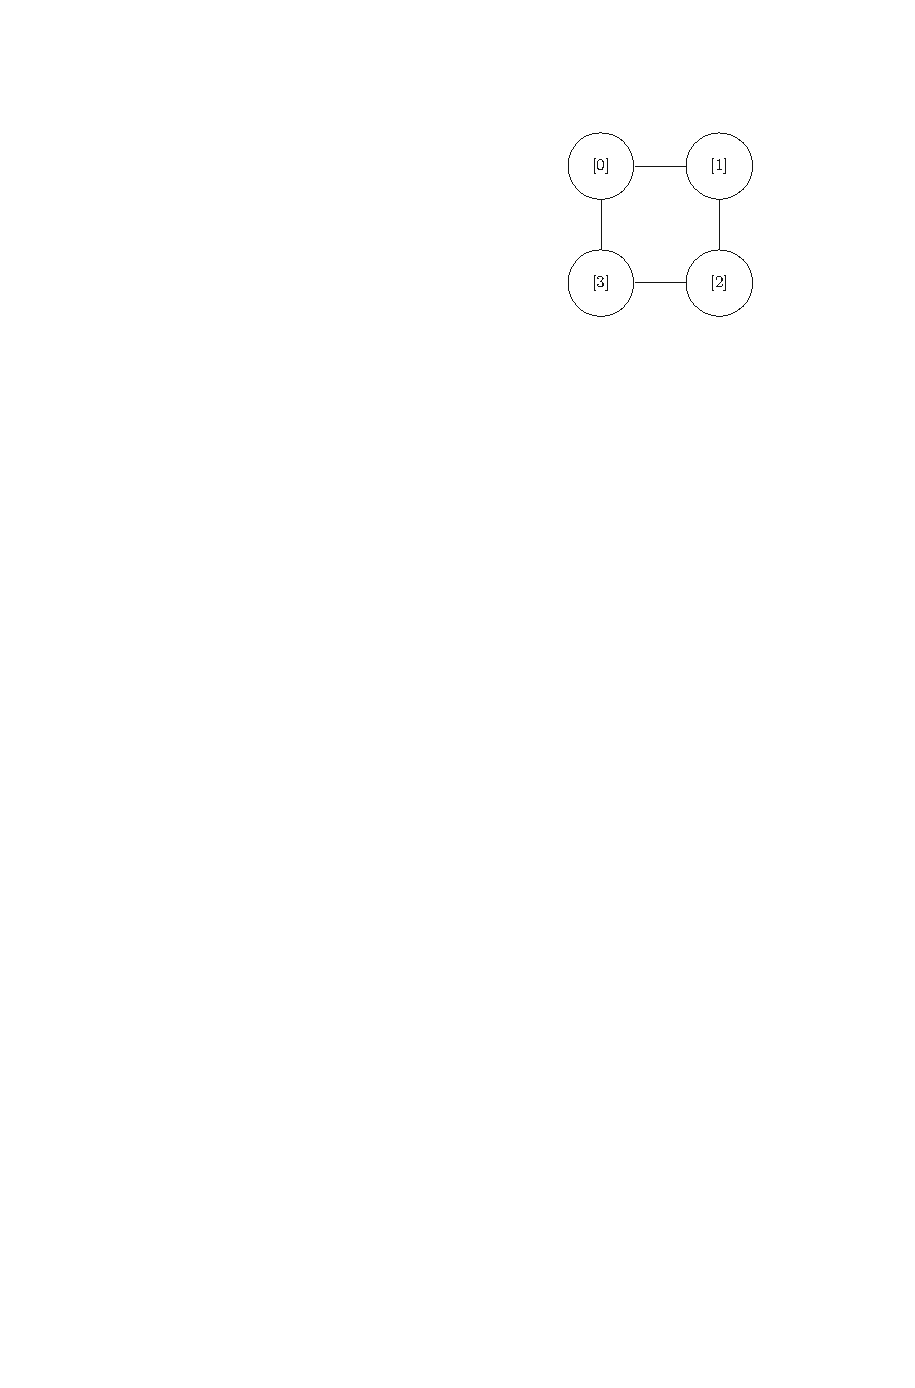
\includegraphics[width=0.25\textwidth]{pictures/Cayley-1.pdf}
\caption{The Cayley graph of $\Z/4\Z$ with respect to $\{\pm[1]\}$}
\label{Cayley graph eg-1}
\end{figure}
\begin{example}
Let $G=\Z/4\Z$ and $S=\{\pm[1]\}$. Then the Cayley graph of $G$ with respect to $S$ is drawn in Figure~\ref{Cayley graph eg-1}. The adjacency matrix of this Cayley graph is given by
\[A=\begin{bmatrix}
0&1&1&0\\
1&0&1&0\\
1&1&0&1\\
0&0&1&0
\end{bmatrix}\]
\end{example}
\begin{figure}[htbp]
\centering
\includegraphics[width=0.45\textwidth]{pictures/Cayley-2.pdf}
\caption{The Cayley graph of $\Z/4\Z$ with respect to $\{\pm[1]\}$}
\label{Cayley graph eg-2}
\end{figure}
\begin{example}
In this example we take $G=\Z/6\Z$ and $S=\{\pm[1],\pm[2]\}$. The resulting Cayley graph can be found in Figure~\ref{Cayley graph eg-2}. The adjacency matrix of this graph is
\[A=\begin{bmatrix}
0&1&1&0&1&1\\
1&0&1&1&0&1\\
1&1&0&1&1&0\\
0&1&1&0&1&1\\
1&0&1&1&0&1\\
1&1&0&1&1&0\\
\end{bmatrix}\]
\end{example}
The graphs we have been considering are Cayley graphs of cyclic groups. Such
graphs have a special name.
\begin{definition}[\textbf{Circulant graph}]
A Cayley graph of $\Z/n\Z$ is called a \textbf{circulant graph} on $n$ vertices.
\end{definition}
The adjacency matrix of a circulant graph is an example of a special type of
matrix known as a circulant matrix.
\begin{definition}
An $n\times n$ circulant matrix is a matrix of the form
\[A=\begin{bmatrix}
a_0&a_1&\cdots&a_{n-2}&a_{n-1}\\
a_{n-1}&a_0&a_{1}&\cdots&a_{n-2}\\
\vdots&a_{n-1}&a_0&\ddots&\vdots\\
a_2&\vdots&\ddots&\ddots&a_{1}\\
a_1&a_2&\cdots&a_{n-1}&a_{0}\\
\end{bmatrix}\]
\end{definition}
Equivalently, a matrix $A$ is circulant if there exists a function $f:\Z/n
Z\to\C$ such that $A_{ij}=f([j]-[i])$. In the above form, one has $a_i=f([i])$ for $0\leq i\leq n-1$. If $S$ is a symmetric subset of $\Z/n\Z$, then the circulant matrix corresponding to the indicator functions $\delta_S$ of $S$ is the adjacency matrix of the Cayley graph of $\Z/n\Z$ with respect to $S$.\par
Our goal is to describe the eigenvalues of the Cayley graph of an abelian group. First we need a lemma about the group algebra $L(G)$.
\begin{lemma}\label{convolution eigen}
Let $G$ be an abelian group and $a\in L(G)$. Define the convolution operator $A:L(G)\to L(G)$ by $A(b)=a\ast b$. Then $A$ is linear and $\chi$ is an eigenvector of $A$ with eigenvalue $\widehat{a}(\chi)$ for all $\chi\in G^\vee$. Consequently, $A$ is a diagonalizable operator.
\end{lemma}
\begin{proof}
Using the distributivity of convolution over addition, it is easy to verify that $A$ is linear. Let $n=|G|$ and suppose that $\chi\in G^\vee$. Observe that
\[\widehat{a\ast\chi}=\ast{a}\cdot\widehat{\chi}=n\widehat{a}\delta_\chi\]
Clearly, one has that
\[(\widehat{a}\cdot n\delta_\chi)(\theta)=\begin{cases}
\widehat{a}(\theta)n&\chi=\theta\\
0&\text{otherwise}
\end{cases}\]
so we conclude
\[\widehat{a}\cdot n\delta_\chi=\widehat{a}(\chi)n\delta_\chi\]
Applying the inverse of the Fourier transform
to $\widehat{a\ast\chi}$ and using that $\widehat{\chi}=n\delta_\chi$, we obtain $a\ast\chi=\widehat{a}(\chi)\chi$, and so $\chi$ is an eigenvector of $A$ with eigenvalue $\widehat{a}(\chi)$.\par
Since $G$ is abelian, the elements of $G^\vee$ form an orthonormal basis of $L(G)$, it follows that $A$ is diagonalizable.
\end{proof}
Lemma~\ref{convolution eigen} is the key ingredient to computing the eigenvalues of the adjacency matrix of a Cayley graph of an abelian group. It only remains to realize the adjacency matrix as the matrix of a convolution operator.
\begin{theorem}
Let $G=\{g_1,\cdots,g_n\}$ be an abelian group and $S\sub G$ a symmetric set. Let $\chi_1,\cdots,\chi_n$ be the irreducible characters of $G$ and let $A$ be the adjacency matrix of the Cayley graph of $G$ with respect to $S$ $($using this ordering for the elements of $G)$. Then:
\begin{itemize}
\item[$(\rmnum{1})$]The eigenvalues of the adjacency matrix $A$ are the real numbers
\[\lambda_i=\sum_{s\in S}\chi_i(s)\]
where $1\leq i\leq n$.
\item[$(\rmnum{2})$]The corresponding orthonormal basis of eigenvectors is given by the vectors $\{v_1,\cdots,v_n\}$ where
\[v_i=\frac{1}{\sqrt{|G|}}(\chi_i(g_1),\cdots,\chi_i(g_n))^T\]
\end{itemize}
\end{theorem}
\begin{proof}
Let $G=\{g_1,\cdots,g_n\}$ and let $\delta_S=\sum_{s\in S}\delta_s$ be the characteristic (or indicator) function of $S$; so
\[\delta_S(x)=\begin{cases}
1&x\in S\\
0&x\notin S
\end{cases}\]
Let $F:L(G)\to L(G)$ be the convolution operator
\[F(b)=\delta_S\ast b\]
Lemma~\ref{convolution eigen} implies that the irreducible characters $\chi_i$ are eigenvectors of $F$ and that the corresponding eigenvalue is
\[\widehat{\delta_S}(\chi_i)=n\langle\delta_S,\chi_i\rangle=\sum_{x\in G}\delta_S(x)\widebar{\chi_i(x)}=\sum_{x\in S}\widebar{\chi_i(x)}\]
where the penultimate equality is obtained by putting $s=x^{-1}$ and using that degree one representations are unitary, whence $\chi_i(x^{-1})=\chi_i(x)$, and that $S$ is symmetric.\par
By the observation
\[\chi_i=\sum_{j=1}^{n}\chi_i(g_j)\delta_{g_j}\]
it follows that if $B$ is the basis $\{\delta_{g_1},\cdots,\delta_{g_n}\}$ for $L(G)$, then the matrix $[F]_B$ of $F$ with respect to this basis has eigenvalues $\lambda_1,\cdots,\lambda_n$ and eigenvectors $v_1,\cdots,v_n$.
The orthonormality of the $v_i$ follows from the orthonormality of the $\chi_i$:
\begin{align*}
\langle v_i,v_j\rangle&=\frac{1}{|G|}\sum_{k=1}^{n}\chi_i(g_k)\widebar{\chi_j(g_k)}=\langle\chi_i,\chi_j\rangle=\begin{cases}
1&i=j\\
0&i\neq j
\end{cases}
\end{align*}
Therefore, it remains to prove that $A=[F]_B$. To this end we compute
\[F(\delta_{g_j})=\delta_S\ast\delta_{g_j}=\sum_{s\in S}\delta_s\ast\delta_{g_j}=\sum_{s\in S}\delta_{sg_j}\]
Recalling that $([F]_B)_{ij}$ is the coefficient of $\delta_{g_j}$ in $F(\delta_{g_j})$, we conclude that
\begin{align*}
([F]_B)_{ij}&=\begin{cases}
1&sg_j=g_i\text{ for some $s\in S$}\\
0&\text{otherwise}
\end{cases}\\
&=\begin{cases}
1&g_ig_j^{-1}\in S\\
0&\text{otherwise}
\end{cases}\\
&=A_{ij}.
\end{align*}
as required.\par
Finally, to verify that $\lambda_i$ is real, we just observe that if $s\in S$, then either $s=s^{-1}$, and so $\chi_i(s)=\chi_i(s^{-1})=\widebar{\chi_i(s)}$ is real, or $s^{-1}\in S$ and $\chi(s)+\chi(s^{-1})=\chi(s)+\widebar{\chi(s)}$ is real.
\end{proof}
Specializing to the case of circulant matrices, we obtain:
\begin{corollary}
Let $A$ be a circulant matrix of degree $n$, which is the adjacency matrix of the Cayley graph of $\Z/n\Z$ with respect to the symmetric set $S$. Then the
eigenvalues of $A$ are
\[\lambda_k=\sum_{[m]\in S}e^{\frac{2\pi ikm}{n}}\]
where $k=0,\cdots,n-1$ and a corresponding basis of orthonormal eigenvectors is given by $v_0,\cdots,v_{n-1}$ where
\[v_k=\frac{1}{\sqrt{n}}(1,e^{\frac{2\pi ik 2}{n}},\cdots,e^{\frac{2\pi ik (n-1)}{n}})^T\]
\end{corollary}
\subsection{Fourier Analysis on Non-abelian Groups}
For a non-abelian group $G$, we have $L(G)\neq Z(L(G))$ and so $L(G)$ is a
non-commutative ring. Therefore, we cannot find a Fourier transform that turns
convolution into pointwise multiplication, as pointwise multiplication is commutative. Instead, we try to replace pointwise multiplication by matrix multiplication. To achieve this, let us first recast the abelian case in a different form.\par
Suppose that $G$ is a finite abelian group with irreducible characters $\chi_1,\cdots,\chi_n$. Then to each function $f:G\to\C$, we can associate its vector of Fourier coefficients. That is, we define $T:L(G)\to\C^n$ by
\[Tf=(n\langle f,\chi_1\rangle,\cdots,n\langle f,\chi_n\rangle)=(\widehat{f}(\chi_1),\cdots,\widehat{f}(\chi_n))\]
The map $T$ is injective by the Fourier inversion theorem because we can recover $\widehat{f}$, and hence $f$, from $Tf$. It is also linear and hence a vector space isomorphism since $\dim L(G)=n$. Now $\C^n$ has the structure of a direct product of rings where multiplication is taken coordinate-wise. The map $T$ is in fact a ring isomorphism since
\[T(a\ast b)=(\widehat{a\ast b}(\chi_1),\cdots,\widehat{a\ast b}(\chi_n))=(\widehat{a}(\chi_1)\widehat{b}(\chi_1),\cdots,\widehat{a}(\chi_n)\widehat{b}(\chi_n))=T(a)T(b)\]
Theorem~\ref{Convolution theorem} can thus be reinterpreted in the following way.
\begin{theorem}
Let $G$ be a finite abelian group of order $n$. Then $L(G)\cong\C^n$.
\end{theorem}
One might guess that this reflects the fact that all irreducible representations of an abelian group have degree one and that, for non-abelian groups, we must replace $\C$ by matrix rings over $\C$. This is indeed the case. So without further ado, let $G$ be a finite group of order $n$ with complete set $\varphi^{(1)},\cdots,\varphi^{(s)}$ of unitary representatives
of the equivalence classes of irreducible representations of $G$. As usual, we put $d_k=\deg\varphi^{(k)}$. The matrix coefficients are the functions $\varphi^{(k)}_{ij}:G\to\C$ given by $\varphi^{(k)}_g=\varphi^{(k)}_{ij}(g))$. Proposition~\ref{repre L(G) basis} tells us that the functions $\sqrt{d_k}\varphi^{(k)}_{ij}$ form an orthonormal basis for $L(G)$.
\begin{definition}[\textbf{Fourier transform}]
Define
\[T:L(G)\to\mathcal{M}_{d_1}(\C)\times\cdots\times\mathcal{M}_{d_k}(\C)\]
by $Tf=(\widehat{f}(\varphi^{(1)}),\cdots,\widehat{f}(\varphi^{(s)}))$ where
\[\widehat{f}(\varphi^{(k)})_{ij}=n\langle f,\varphi^{(k)}_{ij}\rangle=\sum_{g\in G}f(g)\widebar{\varphi^{(k)}_{ij}(g)}\]
We call $Tf$ the Fourier transform of $f$.
\end{definition}
Notice that $Tf$ can be written more succinctly in the form
\[\widehat{f}(\varphi^{(k)})=\sum_{g\in G}f(g)\widebar{\varphi^{(k)}(g)}\]
which is the form that we shall most frequently use.\par
Let us begin our study of non-abelian Fourier analysis with the Fourier inversion theorem.
\begin{theorem}
Let $f:G\to\C$ be a complex-valued function on $G$. Then
\[f=\frac{1}{n}\sum_{i,j,k}d_k\widehat{f}(\varphi^{(k)})\varphi^{(k)}_{ij}\]
where $n=|G|$.
\end{theorem}
\begin{proof}
We compute using the orthonormality of the $\sqrt{d_k}\varphi^{(k)}_{ij}$
\begin{align*}
f=\sum_{i,j,k}\langle f,\sqrt{d_k}\varphi^{(k)}_{ij}\rangle\sqrt{d_k}\varphi^{(k)}_{ij}=\frac{1}{n}\sum_{i,j,k}d_kn\langle f,\varphi^{(k)}_{ij}\rangle\varphi^{(k)}_{ij}=\frac{1}{n}\sum_{i,j,k}d_k\widehat{f}(\varphi^{(k)})_{ij}\varphi^{(k)}_{ij}
\end{align*}
\end{proof}
Next we show that $T$ is a vector space isomorphism.
\begin{theorem}
The map $T:L(G)\to\mathcal{M}_{d_1}(\C)\times\cdots\times\mathcal{M}_{d_s}(\C)$ is a vector space isomorphism.
\end{theorem}
\begin{proof}
It is easy to verify the map $T$ is linear. Since we have
\[\dim L(G)=d_1^2+\cdots+d_s^2=|G|\]
and $T$ is injective, we conclude it is an isomorphism.
\end{proof}
All the preparation has now been completed to show that the Fourier transform
is a ring isomorphism. This leads us to a special case of a more general theorem of Wedderburn that is often taken as the starting point for studying the representation theory of finite groups.
\begin{theorem}
The Fourier transform
\[T:L(G)\to\mathcal{M}_{d_1}(\C)\times\cdots\times\mathcal{M}_{d_k}(\C)\]
is an isomorphism of rings.
\end{theorem}
\begin{proof}
We have already showed $T$ is an isomorphism of vector spaces. Therefore, to show that it is a ring isomorphismit suffices to verify that $T(a\ast b)=Ta\cdot Tb$. In turn, by the definition of multiplication in a direct product, to do this it suffices to establish $\widehat{a\ast b}(\varphi^{(k)})=\widehat{a}(\varphi^{(k)})\cdot\widehat{b}(\varphi^{(k)})$ for $1\leq k\leq s$. The computation is analogous to the abelian case:
\begin{align*}
\widehat{a\ast b}(\varphi^{(k)})&=\sum_{x\in G}(a\ast b)(x)\widebar{\varphi^{(k)}(x)}=\sum_{x\in G}\widebar{\varphi^{(k)}(x)}\sum_{y\in G}a(xy^{-1})b(y)\\
&=\sum_{z\in G}\widebar{\varphi^{(k)}(zy)}\sum_{y\in G}a(z)b(y)\\
&=\sum_{z\in G}\sum_{y\in G}a(z)\widebar{\varphi^{(k)}(z)}b(y)\widebar{\varphi^{(k)}(y)}\\
&=\widehat{a}(\varphi^{(k)})\widehat{b}(\varphi^{(k)})
\end{align*}
This concludes the proof that $T$ is a ring isomorphism.
\end{proof}
\begin{remark}
Note that
\[\widehat{\delta_g}(\varphi^{(k)})=\sum_{x\in G}\delta_g(x)\widebar{\varphi^{(k)}(x)}=\widebar{\varphi^{(k)}(g)}\]
Since the conjugate of an irreducible representation is easily verified to be irreducible, it follows that $T\delta_g$ is a vector whose entries consist of the images of $g$ under all the irreducible representations of $G$, in some order.
\end{remark}